% Symbolic IV: Discovering Structural Equations under Endogeneity
% Working paper. Build: paper\build.cmd (Windows) or bash paper/build.sh; or open in VS Code with LaTeX Workshop.
\documentclass[11pt,a4paper]{article}

\usepackage[T1]{fontenc}
\usepackage[utf8]{inputenc}
\usepackage{lmodern}
\usepackage{microtype}
\usepackage[margin=1.1in]{geometry}
\usepackage{amsmath,amssymb,amsthm}
\usepackage{mathtools}
\usepackage{booktabs}
\usepackage{array}
\usepackage{makecell}
\usepackage{graphicx}
\usepackage{caption}
\usepackage{enumitem}
\usepackage{xcolor}
\usepackage[round,authoryear]{natbib}
\usepackage[colorlinks=true,linkcolor=blue!50!black,citecolor=blue!50!black,urlcolor=blue!50!black]{hyperref}

\graphicspath{{../experiments/phase4/}}
\captionsetup{font=small,labelfont=bf}
\setlist{nosep}
% Let TeX loosen a line slightly rather than run inline mathematics into the margin.
\setlength{\emergencystretch}{2em}
\bibliographystyle{plainnat}

% Results keep the numbering of THEORY.md in the repository (Theorem 1, Proposition 2.1, ...), so the
% statements are named by hand rather than numbered by LaTeX. The optional argument is a label key
% (Theorem1, Proposition2.1, Theorem3(a), ...) that \res links to.
\newenvironment{result}[2][]{\par\medskip\noindent%
  \if\relax\detokenize{#1}\relax\else\phantomsection\label{res:#1}\fi%
  \textbf{#2.}\ \itshape\ignorespaces}{\par\medskip}
% \res{Theorem}{1} prints "Theorem 1" with the number linked to the statement, as Section~\ref{} does.
\DeclareRobustCommand{\resnum}[2]{\hyperref[res:#1#2]{#2}}
\DeclareRobustCommand{\res}[2]{#1~\resnum{#1}{#2}}
\newenvironment{remarks}{\par\medskip\noindent\emph{Remarks.}}{\par\medskip}
\newcommand{\norm}[1]{\lVert #1\rVert}
\newcommand{\bignorm}[1]{\bigl\lVert #1\bigr\rVert}
\newcommand{\abs}[1]{\lvert #1\rvert}
\newcommand{\E}{\mathbb{E}}
\newcommand{\R}{\mathbb{R}}
\newcommand{\Sc}{\mathcal{S}}
\newcommand{\Fc}{\mathcal{F}}
\newcommand{\Hc}{\mathcal{H}}
\newcommand{\Cc}{\mathcal{C}}
\newcommand{\Dc}{\mathcal{D}}
\newcommand{\Gc}{\mathcal{G}}
\newcommand{\Xc}{\mathcal{X}}
\newcommand{\Nc}{\mathcal{N}}
\newcommand{\crit}{\mathrm{crit}}
\newcommand{\pen}{\mathrm{pen}}
\newcommand{\dloc}{d^{\mathrm{loc}}}
\newcommand{\dist}{\mathrm{dist}}
\newcommand{\tr}{\mathrm{tr}}
\newcommand{\AR}{\mathrm{AR}}
\newcommand{\Lip}{\mathrm{Lip}}
\DeclareMathOperator*{\argmin}{arg\,min}
\newcommand{\ind}{\mathbf{1}}
\newcommand{\code}[1]{\texttt{#1}}
% Shrink a table to the text width only when it is wider than that; never enlarge it.
\newcommand{\fittable}[1]{\resizebox{\ifdim\width>\textwidth\textwidth\else\width\fi}{!}{#1}}

\title{Symbolic IV: Discovering Structural Equations under Endogeneity}
\author{Manuel Sanchez\thanks{Independent researcher. ORCID: \href{https://orcid.org/0000-0002-2976-2733}{0000-0002-2976-2733}. E-mail: \href{mailto:manuzrp@gmail.com}{manuzrp@gmail.com}. Code and a replication guide: \url{https://github.com/manuzrpEd/IV_SymbolicRegression}.}}
\date{11 October 2026\\[4pt]\normalsize Preliminary draft. Comments welcome.}

\begin{document}
\maketitle

\begin{abstract}
\noindent Symbolic regression finds the formula that best predicts an outcome, so under endogeneity it returns a formula for the conditional mean, not the structural law. This paper scores the formula search with instrumental-variable moment conditions instead: candidate formulas from cheap generators are refitted by GMM on sieve instruments, selected by a GMM model-selection criterion with a structure penalty, and reported with an Anderson--Rubin confidence set over formulas that says whether the data identify the result. The selection rule is consistent for any generator whose candidates contain the true form, with a finite-sample bound that attributes its failures to weak separation or to fitting moment noise, and the confidence set covers the true form without any rank condition. In a Monte Carlo over five designs and five laws, the method recovers the log, power and two-regressor laws in 92--100\% of runs under confounding and a heteroskedastic first stage, while the squared-error search never recovers the power law under strong endogeneity, and it flags every weak-instrument run as weakly identified or rejected. On the Engel curves of the 1995 Family Expenditure Survey it reproduces the known Working--Leser and quadratic shapes; on Angrist and Krueger's quarter-of-birth instruments it reports weak identification instead of a formula.

\medskip\noindent\textbf{Keywords:} symbolic regression; instrumental variables; nonparametric IV; GMM model selection; weak identification.

\noindent\textbf{JEL:} C14, C26, C52.
\end{abstract}

\newpage

\section{Introduction}

Symbolic regression (SR) searches over mathematical expressions, built from a small set of operators, variables and free constants, for the formula that best predicts an outcome $y$ from regressors $X$ \citep{schmidt2009,udrescu2020,cranmer2023}. Its promise for economics is an interpretable functional form found from the data rather than assumed: a demand curve, an Engel curve, a return to schooling, with elasticities that change with the level, thresholds, and diminishing returns read off the formula. The difficulty is that SR minimizes a prediction loss, so at best it is consistent for the conditional mean $\E[y \mid X]$. In the structural model
\[
y = f_0(X) + u, \qquad \E[u \mid X] \neq 0,
\]
the conditional mean is $f_0(X) + \E[u \mid X]$, and the formula SR returns describes the sum, not the law. In economics almost every regressor of interest is endogenous: prices are set in equilibrium with quantities, schooling is chosen, hours respond to wages, policies are taken up by those who benefit. SR applied to such data \citep{balla2025,rossetti2026} produces convincing formulas that are not causal.

Econometrics has three answers to endogeneity, and each loses something that SR offers. Parametric instrumental-variable (IV) estimation \citep{hansen1982} needs the functional form in advance. Sparse IV over a term library \citep{gautierrose,fanliao2014,linfengli2015,caner2009} selects terms under endogeneity, but only for laws that are linear in their parameters over a dictionary fixed in advance: $a + b\log x$ yes, $a x^{\theta}$ with unknown $\theta$, a kink at an unknown point, or a saturation curve $ax/(b + x)$ no. Nonparametric IV \citep{neweypowell2003,hallhorowitz2005,bck2007,chenpouzo2012} and its machine-learning versions \citep{hartford2017,singh2019,bennett2019,dikkala2020,xu2021} impose nothing on the form but return a curve or a network, not a formula, and the estimation problem is ill-posed. No method searches over free-form formulas while enforcing the conditional moment restriction $\E[y - f(X) \mid Z] = 0$ for an instrument $Z$. This paper fills that gap. What the moment restriction buys is that the formula found is a structural law and not a description of the conditional mean: the data choose the functional form, and the instrument carries the identification. The task is then to show that this can be done consistently, that it works at the sample sizes economists have, and that the method says so when the instruments do not identify the form.

The estimator proposed here has three steps. Candidate formulas are generated cheaply, by any means: a plain squared-error SR search, an SR search distilled from a sieve two-stage least-squares (2SLS) curve, a sparse path over a term library projected on the instruments, and a fixed library of textbook economic shapes with free constants. The constants of every candidate are then refitted by two-step GMM on $K$ sieve instruments, and the formula is selected by a GMM model-selection criterion in the sense of \citet{andrewslu2001}, Hansen's $J$ statistic plus a BIC penalty per constant, to which we add a per-node \emph{structure} penalty that accounts for the search over formula structures. Finally, an identification diagnostic built on the Anderson--Rubin statistic \citep{stockwright2000} reports the first-stage strength, identification-robust intervals for the constants, and the \emph{formula confidence set}: the candidate formulas the data do not reject. The verdict is ``identified'', ``weakly identified'' (with the formulas the data also allow listed) or ``rejected''.

The central finding of the Monte Carlo simulation is that the instrument does its work when formulas are \emph{scored}, not when they are generated. The squared-error search's own pick carries the endogeneity bias, but its list of candidate formulas usually contains the true form, and the moment criterion selects it. Distilling a sieve-2SLS curve gives candidates that select even better, and a fixed library of economic templates gives full coverage of the textbook shapes at no search cost. The expensive alternative, running the SR search itself on the moment criterion, buys nothing that scoring does not.

Section~\ref{sec:theory} gives the selection rule a theory. Bounded constants and bounded formula size turn the ill-posed inverse problem into a choice among finitely many parametric models, and the rule then selects a minimal true formula with probability tending to one for \emph{any} generator whose candidates contain one, with constants at the parametric rate and valid split-sample inference (\res{Theorem}{1}). A finite-sample bound (\res{Theorem}{2}) names the two ways selection fails, a wrong formula the moments barely separate from the truth and a longer formula that fits the moment noise, and shows that the per-node structure penalty is what controls the second as formulas grow. The formula confidence set covers the true form at the nominal level without any rank condition (\res{Proposition}{5}), so the diagnostic reports weak identification, rather than a confident formula, when the instruments do not identify the form. A $J$-point instrument cannot exclude a formula with $J$ or more constants whose moment equations have a solution within the constant bound (\res{Proposition}{4}), and under misspecification the estimator converges to the pseudo-true set, and to any Lipschitz law when the formula size grows with $n$ (\res{Theorem}{3}). The theory thus says what the Monte Carlo shows: once the candidates contain the truth, what decides is how far the moments separate them, not the search that produced them.

Section~\ref{sec:mc} reports a Monte Carlo of 1{,}098 SR searches over five designs (confounding, a heteroskedastic first stage that breaks the control-function approach, simultaneity, a discrete instrument, a weak instrument) and five laws (log, power, kink, saturation, two regressors), against nine baselines: oracle and wrong-form IV, sieve 2SLS, kernel IV, DeepIV, their symbolic distillations, library IV, control-function SR and an SRIT-style causal SR. With strong instruments the method recovers the log, power and two-regressor laws in 92--100\% of runs under confounding and a heteroskedastic first stage, and in 60--92\% under simultaneity and a discrete instrument; the squared-error search never recovers the power law under strong endogeneity, and where it finds the log form its slope is biased by exactly the amount the theory predicts. In the strong-endogeneity design recovery reaches 98--100\% from $n = 5000$ with the structure penalty, while with BIC alone recovery of the power law plateaus at 75--92\% because near-duplicates of the law win. Under the weak instrument recovery is 0--2\%, and the diagnostic flags every run. Section~\ref{sec:apps} applies the method to the Engel curves of the 1995 Family Expenditure Survey sample of \citet{bck2007}, where it reproduces the known shapes and reports no share as identified, and to \citet{angristkrueger1991}, where it reports weak identification instead of a formula, as it should. Section~\ref{sec:budget} shows that a fixed template library raises recovery where the moments separate the law, while an eight-fold search budget raises coverage but not recovery, because more candidates bring more wrong formulas that outscore the truth, the second channel of \res{Theorem}{2} in the data.

The closest related work is of three kinds, and the paper differs from each in one respect. Against sparse IV over a library, discussed above, the search here is over free-form formulas, and the library path becomes one candidate generator among others, whose limit turns out to be coverage rather than the IV logic: it never contains the power, kink or saturation laws. IV in system identification \citep{kuanglin2026,zeiringer2026} corrects coefficients for measurement noise over a fixed library, without external instruments and without a search over structures; here both are present. Causal constraints inside SR \citep{yan_srit,li2026,kacprzyk2024}, theory-constrained SR \citep{kronberger2022,cornelio2023,corywright2024,russeil2024} and sparse identification of dynamics \citep{brunton2016} restrict the inputs, the form or the library under causal sufficiency, ignorability or prior theory, and all still target $\E[y \mid X]$; unobserved confounding handled through instruments, which \citet{yan_srit} state as open, is what this paper adds. The nearest existing route, distilling an NPIV fit into a formula in the manner of \citet{cranmer2020}, is one of our generators, and the Monte Carlo locates its weakness in the selection step, which the criterion proposed here repairs. The econometric tools are standard: the criterion extends the GMM model selection of \citet{andrews1999} and \citet{andrewslu2001} to formula classes, the diagnostic applies \citet{stockwright2000} to a set of candidate formulas, the finite-sample bound uses \citet{tropp2012} and \citet{hsukakadezhang2012}, the misspecified and growing-size results follow the sieve literature \citep{aichen2003,chen2007,chenpouzo2012} and \citet{hallinoue2003}, and inference after selection is by sample splitting, with no uniform claim \citep{leebpotscher2005,berk2013}.

The assumptions are chosen to make the problem a selection problem, and each has a price. The error is additive and mean-independent of the instrument. This is what turns a candidate formula into a vector of moments that the data can score; it is also the form in which demand, Engel and earnings equations are written, and it excludes non-separable models with heterogeneous effects, for which the IV quantile model of \citet{chernozhukovhansen2005} is the natural extension. Constants are bounded and formulas have a maximal size. This turns the ill-posed inverse problem into a choice among finitely many parametric models and buys consistency and finite-sample bounds without a regularization scheme; its price is that rates of convergence for a growing size reduce to a modulus of injectivity on the formula sieve (\res{Proposition}{3.3}) that we do not bound, and bounding it for free-knot splines is the most tractable of the open problems. Two limits of the method itself are documented rather than fixed. A threshold law whose kink the instruments barely move and a backward bend at the edge of the data are almost never selected, because a simpler formula fits the moments equally well and no scoring rule can separate formulas the instruments do not distinguish. These are limits of identification within the formula class, not of the estimator; the diagnostic flags part of them, and the remedy is instruments that move the regressor through the kink or the bend, or far larger samples, not a larger search. Section~\ref{sec:limits} collects these with the remaining open problems.

The rest of the paper is organized as follows. Section~\ref{sec:model} states the model, the formula class and the estimator. Section~\ref{sec:theory} gives the theory, with proofs in Appendix~\ref{app:proofs}. Section~\ref{sec:impl} describes the implementation: the criteria, the candidate generators, the selection rules and the diagnostic. Sections~\ref{sec:mc}--\ref{sec:budget} report the Monte Carlo, the applications and the budget experiment. Section~\ref{sec:limits} concludes with the limits and open problems.

\section{Model, formula class and estimator}
\label{sec:model}

\subsection{Model and identification}

Observations $W_i = (y_i, X_i, Z_i)$, $i = 1, \dots, n$, are i.i.d.\ copies of $W = (y, X, Z)$ with $X \in \Xc \subseteq \R^d$. The model is
\begin{equation}
y = f_0(X) + u, \qquad \E[u \mid Z] = 0, \qquad \E[y^2] < \infty,
\label{eq:model}
\end{equation}
and the target is $f_0$. The error is additive; non-separable models such as $y = w \cdot h$ with heterogeneous $w$ violate this and are out of scope. Write $\norm{\cdot}$ for $L^2$ norms and let $T$ be the conditional-expectation operator $(Th)(z) = \E[h(X) \mid Z = z]$ from $L^2(P_X)$ to $L^2(P_Z)$; it satisfies $\norm{Th} \le \norm{h}$.

Plain SR is biased. At best it is consistent for $\E[y \mid X] = f_0(X) + \E[u \mid X]$. In the baseline Monte Carlo design (Section~\ref{sec:mc}), $X = \exp(\pi Z + v)$ and $u = \rho v + \sigma\varepsilon$, so $\E[u \mid X] = \frac{\rho}{1 + \pi^2}\log X$: for the log law $a + b\log x$ the conditional mean has the right form with a biased slope, $b + \rho/(1 + \pi^2)$; for every other law it has an extra $\log X$ term. Whether an SR search shows that term depends on its size relative to $f_0$; in the Monte Carlo the squared-error search's own pick had the right power form with a 6\% bias in the constant when the term was small, and never had the form when it was large.

Identification is needed only within the formula class. Let $\Fc_L$ be the class defined below; we need only \emph{restricted identification}:
\begin{equation}
f \in \Fc_L, \quad \E[f(X) - f_0(X) \mid Z] = 0 \text{ a.s.} \;\Rightarrow\; f = f_0.
\label{eq:restricted-id}
\end{equation}
Completeness of $X$ given $Z$ \citep{dhaultfoeuille2011} is sufficient but not necessary; the restricted condition can hold with discrete instruments, where full nonparametric identification fails \citep{freybergerhorowitz2015}. Completeness is not testable in general \citep{canaysantosshaikh2013}, so we treat~\eqref{eq:restricted-id} as an assumption and measure how close it is to failing through the separation constants of Section~\ref{sec:theory}. Ill-posedness, which makes nonparametric IV unstable, enters only through how well the instruments separate the true formula from its competitors: over a ball of functions the modulus of continuity of $T^{-1}$ is zero, while over bounded-constant formulas of bounded size it is positive (\res{Lemma}{1}). Expression length alone is not enough for this: with $\sin$ in the operator set, $\sin(cx)$ has four nodes, yet for large $c$ it is exactly the kind of high-frequency function that $\E[\cdot \mid Z]$ barely sees; with the operators used here, a narrow bump $\exp(-c(x - 1)^2)$ plays the same role. That is why the constants are bounded.

\subsection{Formulas}
\label{sec:formulas}

A \emph{tree} $s$ is an expression tree over an alphabet of $m$ symbols: binary and unary operators, the $d$ variables, and a constant placeholder. It has $\ell_s$ nodes and $p_s$ constant placeholders, and defines $f_s(x;\theta)$ for $\theta$ in its parameter set $\Theta_s$. The operators used throughout are $\{+, -, \times, \div, \mathrm{pow}, \log, \exp, \max\}$, with the exponent of a power restricted to a constant or a single variable, and no nested $\exp(\exp(\cdot))$ or $\log(\log(\cdot))$; for one regressor the alphabet has $m = 10$ symbols.

The \emph{parameter set} $\Theta_s$ is a closed subset of $[-C, C]^{p_s}$ on which $f_s(\cdot;\theta)$ is finite on the support of $X$ and Assumption~(A3) below holds; it is compact. Where the formula is finite everywhere, $\Theta_s$ is the whole cube; for $\log(x - c)$ on a support bounded below by $x_{\mathrm{lo}}$ it is $\{c \le x_{\mathrm{lo}} - \eta\}$ for a margin $\eta > 0$. The code discards candidates whose refit gives non-finite residuals, which is the sample version of this restriction. The bound $C$ is required, not cosmetic: without it, oscillating or spiking terms such as $a\sin(bx)$ or $a\exp(-b(x - c)^2)$ with large $b$ can lower the moment criterion by fitting noise in directions the instruments barely see, and the theory needs a compact class.

The \emph{formula class} is built from $\Sc_L$, the set of trees with at most $L$ nodes; $\Fc_s = \{f_s(\cdot;\theta) : \theta \in \Theta_s\}$ and $\Fc_L = \bigcup_{s \in \Sc_L}\Fc_s$. Unary-binary plane trees with $\ell$ nodes are counted by a Motzkin number, which is at most $3^{\ell}$; each node gets one of $m$ labels, so there are at most $(3m)^{\ell}$ trees of size $\ell$ and
\begin{equation}
\log\abs{\Sc_L} \le L\log(3m) + \log 2.
\label{eq:treecount}
\end{equation}

Under (A0) below, $\Sc_0 = \{s : f_0 \in \Fc_s\}$ is the set of true trees, equality being in $L^2(P_X)$; every other tree in $\Sc_L$ is \emph{wrong}: $f_s(\cdot;\theta) \ne f_0$ for every $\theta \in \Theta_s$. The smallest number of constants that can represent $f_0$ is $p_0 = \min_{s \in \Sc_0}p_s$, and the \emph{minimal true trees} are $\Sc_0^{\min} = \{s \in \Sc_0 : p_s = p_0\}$. For $s \in \Sc_0$, the zero set is $\Theta_s^0 = \{\theta \in \Theta_s : f_s(\cdot;\theta) = f_0\}$. $\Sc_0^{\min}$ usually has several elements: $a + b\log x$ and $\log(cx^{b})$ are both minimal trees for the log law. ``Recovering the form'' means selecting \emph{some} element of $\Sc_0^{\min}$. That is exactly the Monte Carlo's criterion: refit the constants of the selected formula to the noise-free $f_0$, then require an exact fit and $p \le p_0$.

The following assumptions are maintained.
\begin{itemize}
\item[(A0)] Well-specified: $f_0 \in \Fc_L$.
\item[(A1)] $\E[u \mid Z] = 0$.
\item[(A2)] Restricted identification: for $f \in \Fc_L$, $T(f - f_0) = 0$ implies $f = f_0$.
\item[(A3)] Regularity: for every $s$ and every $x$, $\theta \mapsto f_s(x;\theta)$ is continuous on $\Theta_s$, and $\sup_{\theta \in \Theta_s}\abs{f_s(x;\theta)} \le F(x)$ with $\E[F(X)^2] < \infty$.
\end{itemize}

\subsection{The estimator}
\label{sec:estimator}

Given a sample criterion $Q_n$ (Section~\ref{sec:criteria}), the estimator works in three steps.
\begin{enumerate}
\item \textbf{Refit.} Each candidate tree $s$ gets $\hat\theta_s \in \argmin_{\theta \in \Theta_s}Q_n(f_s(\cdot;\theta))$; write $\hat Q_s = Q_n(f_s(\cdot;\hat\theta_s))$.
\item \textbf{Select.}
\begin{equation}
\hat s \in \argmin_{s \in \hat\Sc}\ \crit_n(s), \qquad \crit_n(s) = \frac{n\hat Q_s}{\hat\sigma^2} + \pen_n(s), \qquad \pen_n(s) = p_s\kappa_n + w\,\ell_s\log m.
\label{eq:crit}
\end{equation}
Ties go to fewer constants, then fewer nodes.
\item \textbf{Estimate.} $\hat f = f_{\hat s}(\cdot;\hat\theta_{\hat s})$.
\end{enumerate}
The ingredients: $\hat\Sc \subseteq \Sc_L$ is the candidate set, from any generator (Section~\ref{sec:generators}); $\hat\sigma^2 \to_p \sigma_*^2 \in (0, \infty)$ is the scale that turns $nQ_n$ into a $J$ statistic (exactly so with the 2SLS weight under conditional homoskedasticity, or with the efficient weight; \res{Theorem}{1} needs only an $O_p(1)$ bound at the truth, not the $\chi^2$ calibration); $\kappa_n$ is the per-constant penalty, $\ln n$ (BIC), $2.01\ln\ln n$ (HQIC) or $2$ (AIC); and $w \ge 0$ is the weight of the structure term. With $\kappa_n = \ln n$ and $w = 0$ the rule is the MMSC-BIC of \citet{andrewslu2001}, since $J_n - (K - p)\ln n = \crit_n - K\ln n$, with $p$ the number of free constants, not the node count. ``BIC + structure'' is $w = 0.5$, the value used throughout; $w = 1$ did equally well. Section~\ref{sec:theory} explains the role of each term.

The event $\{\hat\Sc \cap \Sc_0^{\min} \ne \emptyset\}$, that the candidates contain a minimal true tree, is called \emph{coverage}. If it fails, the failure is a \emph{search failure}; if it holds and a wrong or non-minimal tree is selected, the failure is a \emph{statistical failure}. Coverage is a property of the generator, not of the selection rule, and the Monte Carlo reports the two separately.

\section{Theory}
\label{sec:theory}

This section states the results; the proofs are in Appendix~\ref{app:proofs}. The numbering (\res{Theorem}{1}, \res{Proposition}{2.1}, \res{Corollary}{2.2}, \dots) is that of the theory file in the repository, so that each statement can be matched to its proof and to the simulations that test it. \res{Theorem}{1} says what happens as $n \to \infty$; \res{Theorem}{2} says when selection works at a given $n$ and why it fails; \res{Proposition}{5} is the identification diagnostic; \res{Proposition}{4} covers discrete instruments; \res{Theorem}{3} covers misspecification and a growing formula size.

\subsection{Identification on a bounded formula class}

\begin{result}[Lemma1]{Lemma 1}
Assume (A3); for (b) and (c) assume also (A2). Minima and infima over empty sets are $+\infty$.
(a) $\theta \mapsto f_s(\cdot;\theta)$ is continuous from $\Theta_s$ into $L^2(P_X)$, so each $\Fc_s$, and therefore $\Fc_L$, is compact.
(b) Every wrong tree has a positive separation $\delta_s := \min_{\theta \in \Theta_s}\norm{T(f_s(\cdot;\theta) - f_0)}^2 > 0$. Hence $\delta_L := \min_{s \notin \Sc_0}\delta_s > 0$.
(c) For every $\varepsilon > 0$,
\[
\omega_L(\varepsilon) := \inf\{\norm{T(f - f_0)}^2 : f \in \Fc_L,\ \norm{f - f_0} \ge \varepsilon\} > 0.
\]
\end{result}

$\omega_L$ is a modulus of injectivity of $T$ at $f_0$ on $\Fc_L$, the squared inverse function of the modulus of continuity of $T^{-1}$ on $T(\Fc_L)$. Over a ball of functions the analogous modulus is zero, which is why nonparametric IV is ill-posed; over bounded-constant formulas of bounded size it is positive. \res{Theorem}{1} uses the same argument with $Q$ in place of $\norm{T(\cdot)}^2$, and \res{Proposition}{5}(c) with the identity-weight criterion. It gives no rate: $\omega_L(\varepsilon)$ can be tiny, and it shrinks as $L$ or $C$ grows. The separation constant $\delta_L$ is the part of this modulus that comes from wrong trees.

\subsection{Criteria}
\label{sec:criteria}

All results use three properties of a sample criterion $Q_n$ and its population limit $Q$:
\begin{itemize}
\item[(C1)] $Q \ge 0$, $Q$ is continuous on $\Fc_L$ in the $L^2$ norm, and for $f \in \Fc_L$: $Q(f) = 0 \iff f = f_0$.
\item[(C2)] $\sup_{f \in \Fc_L}\abs{Q_n(f) - Q(f)} \to_p 0$.
\item[(C3)] $n\,Q_n(f_0) = O_p(1)$.
\end{itemize}

\begin{result}[Lemma2]{Lemma 2}
(a) \emph{Spline GMM.} Fix $K$. The instruments $b(Z) \in \R^K$ have $\E[bb']$ nonsingular, $\E[\norm{b}^2(y^2 + F(X)^2)] < \infty$ and $\E[\norm{b}^2u^2] < \infty$. Let $Q_n(f) = \hat g(f)'\hat W\hat g(f)$ with $\hat g(f) = n^{-1}\sum_i b(Z_i)(y_i - f(X_i))$ and $\hat W$ positive semidefinite for every $n$ (so that $Q_n \ge 0$) with $\hat W \to_p W$ positive definite. With 2SLS weights $\hat W = (n^{-1}\sum_i b_ib_i')^{-1}$ this is the code's $\norm{A'r}^2/n$, and $Q(f) = \norm{\Pi_KT(f_0 - f)}^2$, where $\Pi_K$ projects onto $\mathrm{span}(b)$. Then (C2) and (C3) hold, and (C1) holds if and only if
\begin{itemize}
\item[(A2$_K$)] for $f \in \Fc_L$, $\Pi_KT(f - f_0) = 0$ implies $f = f_0$.
\end{itemize}
(b) \emph{Kernel MMR.} Let the kernel $k$ be bounded ($\sup_zk(z,z) \le \bar\kappa$), continuous on a separable space of instruments (so that its RKHS is separable, \citealp[Lemma 4.33]{steinwartchristmann2008}), and integrally strictly positive definite in the sense of \citet{sriperumbudur2011}, $\iint k\,d\mu\,d\mu > 0$ for every nonzero finite signed Borel measure $\mu$ (the Gaussian kernel qualifies), and let $Q_n(f) = n^{-2}\sum_{i,j}r_ir_j\,k(Z_i, Z_j)$ with $r_i = y_i - f(X_i)$, whose limit is $Q(f) = \E[T(f_0 - f)(Z)\,T(f_0 - f)(Z')\,k(Z, Z')]$ with $Z'$ an independent copy of $Z$. Then (C1) holds under (A2) alone, and (C2)--(C3) hold under (A3) and $\E[y^2] < \infty$.
\end{result}

(A2$_K$) is stronger than (A2), and it fails for discrete instruments once formulas have many constants (Section~\ref{sec:discrete}). The exact kernel criterion of \citet{zhang2020} needs only (A2), while the Nystr\"om approximation, with landmarks drawn independently of the selection sample, is a GMM criterion with $K$ landmark instruments (Appendix~\ref{app:thm2}); in the Monte Carlo kernel instruments were also slightly better at selection (54\% against 51\% recovery). Both criteria share one implementation: precompute an $n \times K$ matrix $A$ from $Z$ and score $\norm{A'r}^2$ (Section~\ref{sec:impl}).

\subsection{Consistency, selection and inference}

\begin{result}[Theorem1]{Theorem 1}
Assume (A0), (A1), (A3), and a nonnegative criterion $Q_n$ satisfying (C1)--(C3). Let $\kappa_n \ge 0$ with $\kappa_n \to \infty$ and $\kappa_n/n \to 0$, let $w \ge 0$ be fixed, and let $\hat\sigma^2 \to_p \sigma_*^2 \in (0, \infty)$. The candidate set $\hat\Sc$ may depend on the data in any way.
(i) If $P(\hat\Sc \cap \Sc_0 \ne \emptyset) \to 1$, then $\norm{\hat f - f_0} \to_p 0$.
(ii) If $P(\hat\Sc \cap \Sc_0^{\min} \ne \emptyset) \to 1$, then $P(\hat s \in \Sc_0^{\min}) \to 1$.
\end{result}

\begin{remarks}
\begin{enumerate}
\item \emph{Little is needed near the truth.} The proof needs no interior true constants, no rank condition and no $\chi^2$ limit; it uses only the $O_p(1)$ bound (C3) at the truth and the linear growth of the criterion for wrong trees. Over-parameterized true trees, whose extra constants may be unidentified \citep{andrewscheng2012}, do no harm to selection: they lose on the penalty.
\item \emph{Penalties.} BIC and HQIC satisfy $\kappa_n \to \infty$ and $\kappa_n/n \to 0$; AIC does not. Under AIC, over-parameterized true trees win with probability that does not vanish: when $s \supset s^*$ are nested and regular in the sense of (A5) below (for $s$ with rank $p_s$ in (c), so that its extra constants are identified), with the same efficient weight (or the 2SLS weight under conditional homoskedasticity), $J_n(s^*) - J_n(s) \to_d \chi^2_{p_s - p_0}$, so with $w = 0$, $P(\crit_n(s) < \crit_n(s^*)) \to P(\chi^2_k > 2k) > 0$ with $k = p_s - p_0$ (with $w > 0$ the threshold is $2k + w(\ell_s - \ell_{s^*})\log m$ and the limit is still positive). The Monte Carlo found AIC the worst rule. The structure term is bounded by $wL\log m$, so it does not affect consistency; its role is in finite samples (\res{Theorem}{2}).
\item \emph{Any generator works.} (ii) holds for every generator whose candidates contain a minimal true tree with probability tending to one. This is the formal version of the Monte Carlo finding that the instrument is needed when formulas are scored, not when they are generated: the plain squared-error front qualifies whenever it covers, while selecting from it by squared error converges to the conditional-mean formula however large $n$ is.
\item \emph{Cross-fitting has no $\kappa_n$.} A criterion evaluated on held-out moments lets over-parameterized true trees tie with minimal ones in the limit; it is consistent for $f$ but not for the minimal tree, and the recovery metric ($p \le p_0$) counts those ties as failures (28\% recovery in the Monte Carlo).
\end{enumerate}
\end{remarks}

The rate and the inference results need a regularity assumption, (A5) (numbered as in the theory file, which has no (A4)), for a tree $s \in \Sc_0^{\min}$ and the GMM criterion of \res{Lemma}{2}(a), whose setting (in particular $\E[\norm{b}^2(y^2 + F(X)^2)] < \infty$) is in force, with (A2$_K$):
\begin{itemize}
\item[(a)] $\Theta_s^0$ is a finite set of interior points of $\Theta_s$ (a singleton for most trees; a sign-symmetric tree such as $(ax)^2$ has two zeros, $\pm a_0$). Write $\theta_{0s}$ for the element of $\Theta_s^0$ nearest to $\hat\theta_s$.
\item[(b)] $f_s(x;\cdot)$ is continuously differentiable on a neighbourhood $\Nc$ of each point of $\Theta_s^0$, with $\E[\norm{b(Z)}^2\sup_{\Nc}\norm{\partial_\theta f_s}^2] < \infty$.
\item[(c)] $G_s := \E[b(Z)\,\partial_\theta f_s(X;\theta)']$ has full column rank $p_0$ at every $\theta \in \Theta_s^0$.
\item[(d)] $\Omega := \E[b(Z)b(Z)'u^2]$ is positive definite.
\end{itemize}

\begin{result}[Corollary1.1]{Corollary 1.1 (parametric rate)}
Under the assumptions of \res{Theorem}{1}(ii), with the GMM criterion of \res{Lemma}{2}(a), (A2$_K$), and (A5) for every $s \in \Sc_0^{\min}$: $\norm{\hat\theta_{\hat s} - \theta_{0\hat s}} = O_p(n^{-1/2})$ on the event $\{\hat s \in \Sc_0^{\min}\}$, whose probability tends to one. If moreover $\norm{f_s(\cdot;\theta) - f_s(\cdot;\theta')} \le \Lambda\norm{\theta - \theta'}$ for $\theta, \theta'$ near $\Theta_s^0$ and every $s \in \Sc_0^{\min}$, then $\norm{\hat f - f_0} = O_p(n^{-1/2})$.
\end{result}

\begin{result}[Theorem1(iii)]{Theorem 1(iii) (inference after selection)}
Split the sample into $A$ (size $n_A$) and $B$ (size $n_B = n - n_A$), $n_A/n \to a \in (0,1)$, by a rule that does not depend on the data. Compute $\hat s$ on $A$ only: the candidate generator, the scale $\hat\sigma^2$ and the refits that the selection uses all run on $A$ alone (a randomized search may also use randomization independent of the data). On $B$, estimate the constants of $\hat s$ by two-step efficient GMM with fixed $K$; call the result $\tilde\theta$. Assume the conditions of (ii) on $A$, (A2$_K$), the setting of \res{Lemma}{2}(a), and (A5) with $\Theta_s^0$ a singleton $\{\theta_{0s}\}$ for every $s \in \Sc_0^{\min}$ (for a sign-symmetric tree such as $(ax)^2$ with $a_0 > 0$, restrict $\Theta_s$ to $a \ge 0$). Then, with $\hat V$ the usual estimator of $V_{\hat s} = (G_{\hat s}'\Omega^{-1}G_{\hat s})^{-1}$,
\[
\hat V^{-1/2}\sqrt{n_B}\,(\tilde\theta - \theta_{0\hat s}) \to_d N(0, I_{p_0}), \qquad J_B \to_d \chi^2_{K - p_0}\quad (K > p_0).
\]
With (A5)(c) dropped and the other assumptions kept (in particular (A5)(d), which makes $\Omega$ invertible), the Anderson--Rubin statistic $\AR_B(\theta) = n_B\,\hat g_B(\theta)'\hat\Omega_B(\theta)^{-1}\hat g_B(\theta)$, with the continuously-updated weight of Section~\ref{sec:prop5} computed on $B$, at $\theta = \theta_{0\hat s}$ converges to $\chi^2_K$, so $\{\theta : \AR_B(\theta) \le \chi^2_{K,1-\alpha}\}$ covers $\theta_{0\hat s}$ with probability tending to $1 - \alpha$ \citep{stockwright2000}.
\end{result}

The result is pointwise in the data-generating process, not uniform \citep{leebpotscher2005}. The single zero matters: with several zeros the global GMM estimator chooses among the local minimizers by their $J$ statistics, a data-dependent choice under which the studentized statistic is a mixture whose limit need not be normal. Different minimal trees parameterize $f_0$ differently, so the targets to report are tree-invariant: $f_0(x)$ at given points, or elasticities, by the delta method. Two kinds of weak identification must be distinguished: selection needs the \emph{formula} to be strongly identified ($\delta_s$ large relative to $\kappa_n/n$, so that $n\delta_s/\sigma^2$ exceeds the penalty gap in condition (I) of \res{Proposition}{2.1}), while inference about constants can tolerate weakly identified \emph{constants} through AR sets. Under weak instruments it is the first that fails (\res{Theorem}{2}), and \res{Proposition}{5} is the statement that holds without any rank condition. Section~\ref{sec:mc-theory} checks the coverage of these intervals on fresh samples against same-sample inference after selection.

\subsection{A confidence set for the formula}
\label{sec:prop5}

Selection and the intervals of \res{Theorem}{1(iii)} assume that the formula is identified. Under a weak instrument the selection returns a wrong formula with a good fit, and nothing in the output says so. The Anderson--Rubin statistic is valid without any rank condition, so it can be turned into a diagnostic. Take GMM instruments $b(Z) \in \R^K$ with $K$ fixed, $\E[\norm{b}^2u^2] < \infty$ and $\Omega := \E[bb'u^2]$ positive definite. For a tree $s$ and $\theta \in \Theta_s$,
\[
\AR_s(\theta) := n\,\hat g(s,\theta)'\hat\Omega_s(\theta)^{-1}\hat g(s,\theta), \qquad \hat\Omega_s(\theta) := \frac1n\sum_ib(Z_i)b(Z_i)'\bigl(y_i - f_s(X_i;\theta)\bigr)^2,
\]
the weight being evaluated at the same $\theta$ (the continuously-updated objective), with $\AR_s(\theta) := +\infty$ where $\hat\Omega_s(\theta)$ is singular. The \emph{S statistic} of a tree is $S_s := \inf_{\theta \in \Theta_s}\AR_s(\theta)$ \citep{stockwright2000} (an infimum: with the $+\infty$ convention the minimum need not be attained), and the \emph{formula confidence set} of a candidate set $\hat\Sc$ is
\begin{equation}
\Cc_\alpha := \{s \in \hat\Sc : S_s \le \chi^2_{K,1-\alpha}\}.
\label{eq:confset}
\end{equation}

\begin{result}[Proposition5]{Proposition 5}
(a) \emph{Coverage, without identification.} Under (A1) and the setting above, for every true tree $s_0 \in \Sc_0$ and $\theta_0 \in \Theta_{s_0}^0$, $\AR_{s_0}(\theta_0) \to_d \chi^2_K$. Hence, for any candidate set $\hat\Sc$, data-dependent or not,
\[
\limsup_nP\bigl(s_0 \in \hat\Sc,\ s_0 \notin \Cc_\alpha\bigr) \le \alpha.
\]
Neither (A2), nor (A2$_K$), nor a rank condition is used.
(b) \emph{Detection of statistical failures.} Let $E$ be the event that the selected tree $\hat s$ is wrong while $s_0 \in \hat\Sc$. Then $\limsup_nP(E \cap \{s_0 \notin \Cc_\alpha\}) \le \alpha$: given $E$, the miscoverage is at most $(\alpha + o(1))/P(E)$.
(c) \emph{Link to identification.} Assume (A3), (A2$_K$), $\sup_z\norm{b(z)} \le \zeta_K$ and (C2) for the identity-weight criterion. Then the set of functions the data do not reject, $\Gc_\alpha := \{f_s(\cdot;\theta) : s \in \Sc_L,\ \theta \in \Theta_s,\ \AR_s(\theta) \le \chi^2_{K,1-\alpha}\}$, satisfies $\sup_{f \in \Gc_\alpha}\norm{f - f_0} \to_p 0$. Without (A2$_K$) nothing forces it to shrink; its width is what the diagnostic measures.
\end{result}

Part (b) is a joint, not a conditional, statement, because $E$ and $\{\AR_{s_0}(\theta_0) > \chi^2_{K,1-\alpha}\}$ are driven by the same sample; it is informative when $E$ is not rare. In the 630 Monte Carlo runs of Section~\ref{sec:mc-ident}, $E$ occurred 146 times and $\Cc_\alpha$ contained $s_0$ in 145 of them. When $s_0 \in \Cc_\alpha$ is a tree of a form different from $\hat s$'s, the diagnostic reports it as ``a formula the data also allow'' when its S-minimizing fit differs from $\hat f$ by more than $\tau$ standard deviations of $\hat f$, in a trimmed root mean square that discards the 5\% largest differences; the scale is floored at a tenth of the standard deviation of $y$. Near-duplicates within $\tau$ are not reported, by design: the function is then identified even though the tree is not minimal. The implementation adds two guards against a weakness of the robust weight, which discounts exactly the observations a formula misfits most: a sample envelope on the constants and a winsorized weight with a slowly growing cap; Appendix~\ref{app:prop5} states the condition each needs and what it costs. The report returns a verdict: \emph{rejected} when the selected formula fails its own S test ($S_{\hat s} > \chi^2_{K,1-\alpha}$); \emph{weakly identified} when some AR interval of its constants reaches the constant bound, or $\Cc_\alpha$ contains a formula more than $\tau$ away from $\hat f$ (the formulas are listed); \emph{identified} otherwise. It also reports the first-stage $F$ of (log) $X$ on the instruments and the Wald and AR intervals of each constant. A search failure, where no candidate has the true form, is detected only if every candidate fails its S test; if a wrong formula fits the moments, the report says ``identified'' and is wrong about the tree, though usually not about the function.

\subsection{A finite-sample selection bound}
\label{sec:thm2}

\res{Theorem}{2} says when selection works at a given $n$, and why the two failures seen in the Monte Carlo happen: (I) a wrong formula that the instruments cannot tell apart from $f_0$ wins (weak separation), and (II) a formula with extra constants or nodes wins by fitting moment noise (the contrived winners).

The bound is stated in the simplest setting with explicit constants, Setting (F).
\begin{itemize}
\item[(F1)] \emph{Instruments.} GMM with fixed $K$ and population-orthonormal instruments: $\E[bb'] = I_K$ and $\sup_z\norm{b(z)} \le \zeta_K$, so $\zeta_K \ge \sqrt K$. The criterion is $Q_n(s,\theta) = \norm{\hat g(s,\theta)}^2$ with identity weight. The code orthonormalizes on the sample instead; \res{Corollary}{2.5} covers that.
\item[(F2)] \emph{Errors.} $\E[u \mid Z] = 0$ and $\E[e^{\lambda u} \mid Z] \le e^{\lambda^2\bar\sigma^2/2}$ for all $\lambda$. The $J$ statistic is $J_n(s) = (n/\sigma^2)\min_\theta Q_n(s,\theta)$ with a fixed normalization $\sigma^2 > 0$, so that the selection criterion is $\crit_n(s) = J_n(s) + \pen_n(s)$ with $\sigma^2$ in place of the estimated scale of~\eqref{eq:crit} (\res{Corollary}{2.5} treats an estimated scale); write $\nu := \bar\sigma^2/\sigma^2$.
\item[(F3)] \emph{Formula class.} For all $s$, $\theta, \theta'$ and $x$: $\abs{f_s(x;\theta) - f_0(x)} \le M$ and $\abs{f_s(x;\theta) - f_s(x;\theta')} \le \Lambda\norm{\theta - \theta'}_\infty$.
\end{itemize}
(F3) needs a bounded class on the support of $X$; the Monte Carlo designs have lognormal regressors, so for them it is an idealization that holds after truncating the support.

Some notation is needed. The population moments are $g(s,\theta) := \E[b(Z)(f_0 - f_s(\cdot;\theta))(X)]$, so $\norm{g(s,\theta)}^2 = \norm{\Pi_KT(f_s(\cdot;\theta) - f_0)}^2$, and the separation of tree $s$ at this $K$ is $\delta_s := \min_\theta\norm{g(s,\theta)}^2$, positive for wrong trees under (A2$_K$). Writing $\pen(s) := \pen_n(s)$ for the fixed $n$, the penalty gap is $\pi_s := \pen(s) - \overline{\pen}_0$, where $\overline{\pen}_0 := \max_{s' \in \Sc_0^{\min}}\pen(s')$ is the largest penalty of a minimal true tree (the worst case). The moment noise at the truth is $U := \sqrt n\,\bar u/\sigma$ with $\bar u := n^{-1}\sum_ib(Z_i)u_i$; for every $s^* \in \Sc_0^{\min}$, $J_n(s^*) \le \norm{U}^2$. The empirical-process part is $E_s(\theta) := \sqrt n\,(P_n - P)[b(Z)(f_0 - f_s(\cdot;\theta))(X)]/\sigma$, so that for every $s$ and $\theta$
\begin{equation}
\frac{\sqrt n\,\hat g(s,\theta)}{\sigma} = U + \frac{\sqrt n\,g(s,\theta)}{\sigma} + E_s(\theta).
\label{eq:decomp}
\end{equation}

\begin{result}[Proposition2.1]{Proposition 2.1 (deterministic core)}
Assume (A3) and (F1)--(F3). Let $s \notin \Sc_0^{\min}$, and suppose $\norm{U} \le z$ and $\sup_{s,\theta}\norm{E_s(\theta)} \le d$. Then $\crit_n(s) > \crit_n(s^*)$ for every $s^* \in \Sc_0^{\min}$ if either condition holds:
\begin{itemize}
\item[(I)] Separation: $\sqrt{n\delta_s}/\sigma > 2z + d + \sqrt{(-\pi_s)_+}$.
\item[(II)] Complexity: $\pi_s > W_s^2 + 2z\,\dloc_s$,
\end{itemize}
where, with $r := 2z + d$, $\Theta_s(r) := \{\theta \in \Theta_s : \sqrt n\norm{g(s,\theta)}/\sigma \le r\}$ is the localized set of constants, $\Dc_s(r) := \{g(s,\theta)/\norm{g(s,\theta)} : \theta \in \Theta_s(r),\ g(s,\theta) \ne 0\}$ the localized directions, $W_s := \sup_{v \in \Dc_s(r)}\langle -U, v\rangle_+$ (or $0$ if $\Dc_s(r)$ is empty), and $\dloc_s \ge 0$ any bound with $\dloc_s \ge \sup_{\theta \in \Theta_s(r)}\norm{E_s(\theta)}$. Moreover $W_s \le \norm{P_{V_s}U}$, where $V_s := \mathrm{span}\,\Dc_s(r)$.
\end{result}

The proof uses $d$ only through $\sup_\theta\norm{E_s(\theta)}$ for the tree at hand, so $d$ and $r$ may be tree-specific; \res{Corollary}{2.2} uses that. The concentration inequalities that turn \res{Proposition}{2.1} into a probability statement are collected in \res{Lemma}{3} (Appendix~\ref{app:thm2}): a matrix Bernstein bound for the sample second moment of the instruments \citep{tropp2012}, the quadratic-form bound of \citet{hsukakadezhang2012} for $\norm{U}^2$ and for its projections, and a covering argument with McDiarmid's inequality for the empirical process. They define, for a level $t > 0$,
\[
\varepsilon_n(t) := \sqrt{\frac{2\zeta_K^2(t + \log 2K)}{n}} + \frac{2(\zeta_K^2 + 1)(t + \log 2K)}{3n}, \qquad z_t^2 := \nu(1 + \varepsilon_n(t))(K + 2\sqrt{Kt} + 2t).
\]

\begin{result}[Theorem2]{Theorem 2}
Assume (A0), (A1), (A2$_K$) and (F1)--(F3). Fix $t > 0$, let $t_L := t + \log\abs{\Sc_L}$, and define
\[
d_t := \frac{M}{\sigma}\Bigl[\sqrt K + 2\zeta_K + \zeta_K\sqrt{8\bigl(t_L + p_{\max}\log(1 + 2C\Lambda\sqrt n/M)\bigr)}\Bigr], \qquad r_t := 2z_t + d_t,
\]
where $p_{\max} := \max_{s \in \Sc_L}p_s$. For each tree $s$, with the localized set $\Theta_s(r_t)$ and directions $\Dc_s(r_t)$ of \res{Proposition}{2.1}, let $M_s := \sup\{\abs{f_s(x;\theta) - f_0(x)} : x \in \Xc,\ \theta \in \Theta_s(r_t)\}$, $k_s := \dim\mathrm{span}\,\Dc_s(r_t) \le K$, and
\[
\dloc_{s,t} := \frac{M_s}{\sigma}\Bigl[\sqrt K + 2\zeta_K + \zeta_K\sqrt{8\bigl(t_L + p_s\log(1 + 2C\Lambda\sqrt n/M_s)\bigr)}\Bigr],
\]
with $M_s := 0$ when $\Theta_s(r_t)$ is empty, $\dloc_{s,t} := 0$ when $M_s = 0$, and $k_s := 0$ when $\Dc_s(r_t)$ is empty. There is an event of probability at least $1 - 5e^{-t}$ on which, for any candidate set $\hat\Sc \subseteq \Sc_L$ (possibly data-dependent) that contains some $s^* \in \Sc_0^{\min}$, the selected tree is minimal and true, provided every $s \in \Sc_L \setminus \Sc_0^{\min}$ satisfies (I) or (II):
\begin{itemize}
\item[(I)] Separation: $n\delta_s/\sigma^2 > \bigl(2z_t + d_t + \sqrt{(-\pi_s)_+}\bigr)^2$.
\item[(II)] Complexity: $\pi_s > \nu\,(1 + \varepsilon_n(t))\bigl(k_s + 2\sqrt{k_st_L} + 2t_L\bigr) + 2z_t\,\dloc_{s,t}$.
\end{itemize}
Consequently
\[
P(\hat s \notin \Sc_0^{\min}) \le \underbrace{5e^{-t}}_{\text{statistical failure}} + \underbrace{P(\hat\Sc \cap \Sc_0^{\min} = \emptyset)}_{\text{search failure}}.
\]
\end{result}

\res{Theorem}{2} reads as follows. A wrong tree loses if it is separated from $f_0$ by more than the noise plus the penalty it saves (I); a longer or more heavily parameterized tree loses if the penalty it pays exceeds the moment noise it can fit (II). A tree that meets neither condition can win: wrong trees whose separation is small \emph{and} that are no bigger than the minimal true trees, which are the simpler wrong formulas under weak instruments and the same-size near-duplicates when $w = 0$. With $K$ and $L$ fixed, $z_t = O(1)$ and $d_t = O(\sqrt{\log n})$, the latter from the covering term, so (I) holds for a wrong tree as soon as
\begin{equation}
\frac{n\delta_s}{\sigma^2} > 2(p_0 - p_s)_+\kappa_n + 2w(\bar\ell_0 - \ell_s)_+\log m + 2(2z_t + d_t)^2,
\label{eq:margin}
\end{equation}
where $\bar\ell_0 := \max_{s^* \in \Sc_0^{\min}}\ell_{s^*}$; $d_t^2 = O(\log n)$ is of the \emph{same} order as $\kappa_n = \ln n$. So the finite-sample condition is the population comparison $n\delta_s/\sigma^2$ against the penalty saved, plus deviation terms of the same order with explicit constants. The population comparison alone, the margin $n\delta_s/\sigma^2 - (p_0 - p_s)\kappa_n$, is what the Monte Carlo computes for every cell (Section~\ref{sec:mc-grid}): among runs whose candidates contained the true form, recovery was 74\% where the margin is positive and 23\% where it is not. For over-parameterized true trees $\delta_s = 0$, so only (II) can exclude them; as $n$ grows the localized set shrinks to the zero set and, if the moment map is regular there (Appendix~\ref{app:thm2}), $\dloc_{s,t} \to 0$; for a true tree linear in its constants $k_s \le p_s$ exactly, so, with $w = 0$ or $\ell_s \ge \bar\ell_0$, (II) holds if $(p_s - p_0)\kappa_n > \nu(1 + \varepsilon)(p_s + 2\sqrt{p_st_L} + 2t_L) + o(1)$: \res{Theorem}{1}(ii) with explicit sample sizes. For trees nonlinear in $\theta$ the bound $k_s \le p_s$ fails at finite $n$; a first-order version holds with $p_s$ replaced by the dimension of the Jacobian span over the zero set, which is at most $p_s$ for a single zero but can reach $K$ when a constant is unidentified at the truth (Appendix~\ref{app:thm2}). The term $2\nu t_L \approx 2\nu(t + L\log 3m)$ is the price of the union bound over all trees; the next corollary is about it.

\begin{result}[Corollary2.2]{Corollary 2.2 (why a structure term)}
Replace the uniform union bounds in \res{Theorem}{2} by weights proportional to $(3m)^{-\ell_s}/L$, so that $t_L$ becomes the tree-specific $t_s := t + \log L + \ell_s\log(3m)$ in every bound concerning tree $s$. Then (II) holds if
\begin{multline*}
(p_s - p_0)\kappa_n + w(\ell_s - \bar\ell_0)\log m \\ > \nu(1 + \varepsilon_n(t))(2k_s + 3t + 3\log L) + 3\nu(1 + \varepsilon_n(t))\,\ell_s\log(3m) + 2z_t\,\dloc_{s,t_s},
\end{multline*}
and if $w \ge 3\nu(1 + \varepsilon_n(t))\log(3m)/\log m$, the terms in $\ell_s$ cancel: (II) holds whenever $(p_s - p_0)\kappa_n > w\bar\ell_0\log m + \nu(1 + \varepsilon_n(t))(2k_s + 3t + 3\log L) + 2z_t\dloc_{s,t_s}$, a condition that depends on the size of $s$ only through $k_s$ and $\dloc_{s,t_s}$, and on $L$ only through $3\log L$ and the level $t_s$, which enters $\dloc_{s,t_s}$ and the radius $r_{s,t}$ that defines $k_s$ and $M_s$.
\end{result}

The corollary fixes the direction of the structure term, not its weight. With one regressor, $m = 10$, $n = 2000$, $K = 13$, $\zeta_K = \sqrt K$, $\nu = 1$ and $t = 3$, it asks for $w \gtrsim 5.8$, and the leftover term $w\bar\ell_0\log m$ is about $80$ for the log law: nothing is certified at $n = 2000$ for trees of any size, because the union bound over all $(3m)^{\ell}$ trees of each size, with the explicit constants of \res{Lemma}{3}, is vacuous there; without the term the picture is the same with the size of the wrong tree in place of $\bar\ell_0$. The same $w$ enters channel (I) against wrong trees shorter than the true one, so a large $w$ manufactures the ``simpler wrong formula wins'' failure. In the data the structure term raised pooled recovery from 51\% to 60\%, and to 98--100\% from $n = 5000$, with $w = 0.5$ and $w = 1$ doing equally well; what it fixed were same-size near-duplicates of the law ($\pi_s = 0$ when $w = 0$, $\delta_s \approx 0$), the case that falls under neither channel. The data support the direction of the structure term and a weight ten times smaller than the bound asks for.

\begin{result}[Corollary2.3]{Corollary 2.3 (candidates from a separate sample)}
Suppose $\hat\Sc$ is generated on data independent of the selection sample. Conditionally on $\hat\Sc$, \res{Theorem}{2} holds with every union bound running over $\hat\Sc$ instead of $\Sc_L$: $\log\abs{\Sc_L}$ becomes $\log\abs{\hat\Sc}$ in $t_L$.
\end{result}

Had the Monte Carlo candidates come from an independent sample, the union bound would run over a median of 28 pooled candidates per run (Section~\ref{sec:mc-grid}), $\log\abs{\hat\Sc} \approx 3.3$, instead of the bound $\log\abs{\Sc_{15}} \le 52$. But generating on one half and selecting on the other halves the selection sample, so $n\delta_s$ in (I) halves too. Section~\ref{sec:mc-split} tests the trade-off: the mechanism is real, but full-sample selection with the structure term recovers more.

\begin{result}[Proposition2.4]{Proposition 2.4 (perturbed weights)}
Let $\hat W$ be a symmetric matrix, possibly data-dependent, with $\lambda_-\sigma^{-2}I_K \preceq \hat W \preceq \lambda_+\sigma^{-2}I_K$, $0 < \lambda_- \le \lambda_+$, and let the selection use $\tilde J_n(s) := n\min_\theta\hat g(s,\theta)'\hat W\hat g(s,\theta)$. Under the hypotheses of \res{Proposition}{2.1}, with the localization radius $r' := z(1 + \sqrt{\lambda_+/\lambda_-}) + d$ in place of $r$, the conclusion of \res{Proposition}{2.1} holds for the perturbed criterion if either
(I$'$) $\sqrt{n\delta_s}/\sigma > z + d + \sqrt{(\lambda_+/\lambda_-)z^2 + (-\pi_s)_+/\lambda_-}$, or
(II$'$) $\pi_s > (\lambda_+ - \lambda_-)z^2 + \lambda_-(W_s^2 + 2z\,\dloc_s)$.
\end{result}

\begin{result}[Corollary2.5]{Corollary 2.5 (the code's criterion)}
The code uses sample-orthonormalized instruments, $\hat W = \hat\Sigma^{-1}/\sigma^2$ with $\hat\Sigma := n^{-1}\sum_ib(Z_i)b(Z_i)'$. On the event $\norm{\hat\Sigma - I_K} \le \varepsilon := \varepsilon_n(t) < 1$, $\hat W$ satisfies the sandwich with $\lambda_- = (1 + \varepsilon)^{-1}$ and $\lambda_+ = (1 - \varepsilon)^{-1}$, so \res{Theorem}{2} holds for this criterion, with (I$'$)--(II$'$) in place of (I)--(II) and the localization radius $r'_t := z_t(1 + \sqrt{\lambda_+/\lambda_-}) + d_t$ in place of $r_t$ in $M_s$, $k_s$, $\dloc_{s,t}$ and the events of its proof, on an event of probability at least $1 - 5e^{-t}$. If the normalization is an estimated scale $\hat\sigma^2$ common to all candidates with $P(\abs{\hat\sigma^2/\sigma^2 - 1} > \eta_n(t)) \le e^{-t}$, $\eta_n(t) < 1$, $\eta_n(t) \to 0$, then $\lambda_\mp$ are multiplied by $(1 \pm \eta)^{-1}$, in $r'_t$ as well, on a sixth event and the probability becomes $1 - 6e^{-t}$. The perturbation is $\lambda_+ - \lambda_- \approx 2(\varepsilon + \eta)$ in (II$'$) and a factor $\lambda_+/\lambda_- \approx 1 + 2(\varepsilon + \eta)$ on $z^2$ in (I$'$); $\varepsilon_n(t)$ is of order $\sqrt{\zeta_K^2\log K/n}$.
\end{result}

For a fixed positive definite weight $W$, such as the efficient $\Omega^{-1}$ under heteroskedasticity, \res{Theorem}{2} goes through with the instruments rotated to $W^{1/2}b$ and the constants changed accordingly; the estimation error of an efficient weight, and the exact (non-Nystr\"om) kernel criterion, which is a degenerate V-statistic at the truth, are left open (Section~\ref{sec:limits}). The constants of \res{Theorem}{2} are explicit but not optimized; with heavy-tailed errors the tails become polynomial; and for wrong trees with small $\delta_s$ the localized set can contain parameters whose functions are far from $f_0$ but have small moments, the ill-posed directions, so $M_s$ stays large and (II) is loose. Those are the hard cases, and no general improvement should be expected.

\subsection{Discrete instruments}
\label{sec:discrete}

Let $Z$ take $J$ values $z_1, \dots, z_J$ with $P(Z = z_j) > 0$, and write $\mu(h) := (\E[h(X) \mid Z = z_j])_{j=1}^J \in \R^J$. Every function of $Z$ is a step function, so at most $J$ instruments are effective, and with the saturated basis $\Pi_KTh = 0$ if and only if $\mu(h) = 0$.

\begin{result}[Proposition4]{Proposition 4}
(a) \emph{Linear families.} Let $f_s(x;\theta) = \sum_{k=1}^p\theta_k\psi_k(x)$ with $f_0 \notin \Fc_s$. Suppose $\Psi\theta = \mu(f_0)$ has a solution $\theta \in \Theta_s$, where $\Psi = [\E(\psi_k(X) \mid Z = z_j)]$ is the $J \times p$ matrix of the family; when $\Psi$ has rank $J$ (so $p \ge J$) the equation is solvable in $\R^p$ for every $f_0$, and the assumption is that a solution lies in $\Theta_s$. Then (A2$_K$) fails: $f_s(\cdot;\theta) \ne f_0$, yet $\mu(f_s(\cdot;\theta) - f_0) = 0$.
(b) \emph{General families.} Let $\bar\theta$ be interior to $\Theta_s$ and suppose $\theta \mapsto \mu(f_s(\cdot;\theta))$ is $C^1$ near $\bar\theta$ with Jacobian of rank $J$ there (so $p_s \ge J$). Then there is $r > 0$, determined by the tree, the design, $\bar\theta$ and $\Theta_s$ and not by $f_0$, such that every law $f_0$ with $\norm{\mu(f_s(\cdot;\bar\theta) - f_0)} < r$ satisfies $\mu(f_s(\cdot;\theta) - f_0) = 0$ for some $\theta \in \Theta_s$: whenever $s$ is wrong for such an $f_0$, the criterion is exactly zero at a wrong formula.
\end{result}

With a $J$-point instrument, a wrong tree with $J$ or more constants whose moment equations have a solution in its parameter set has $\delta_s = 0$ and cannot be excluded by the moments (the constant bound can block the solution, as for the log law in Section~\ref{sec:mc-discrete}); only the penalty can exclude it, through channel (II) of \res{Theorem}{2}. A practical rule is to cap formulas at $J - 1$ constants when the instrument is discrete; the SVD orthonormalization of the instruments already reduces $K$ to $J$, so the degrees of freedom of the criterion are right. Whether a wrong tree with \emph{fewer} than $J$ constants is generically identified is a transversality statement that we state as \res{Conjecture}{4(c)} in Appendix~\ref{app:prop4} and leave open (Section~\ref{sec:limits}). Section~\ref{sec:mc-discrete} shows \res{Proposition}{4} in the data: with a four-point instrument, a wrong four-constant formula sets the criterion to $10^{-33}$--$10^{-32}$ for three of the four one-regressor laws while missing $f_0$ by 0.12--0.42 standard deviations.

\subsection{Misspecification and growing formula size}
\label{sec:thm3}

\begin{result}[Theorem3(a)]{Theorem 3(a) (fixed $L$, misspecified law)}\label{res:Theorem3}
Drop (A0) and (A2). Assume (A3), $f_0 \in L^2(P_X)$, (C2), $Q$ continuous on $\Fc_L$, $\kappa_n \ge 0$ with $\kappa_n/n \to 0$, and $\hat\sigma^2 = O_p(1)$. Let $Q^* := \min_{f \in \Fc_L}Q(f)$ and $\Fc^* := \argmin_{\Fc_L}Q$, which is nonempty and compact. Suppose $\hat\Sc$ contains, with probability tending to one, a tree of some $f^* \in \Fc^*$. Then $Q(\hat f) \to_p Q^*$ and $\inf_{f \in \Fc^*}\norm{\hat f - f} \to_p 0$.
\end{result}

Under misspecification the pseudo-true set depends on the instrument basis, on $K$ and on the weight \citep{hallinoue2003}: no formula is best independently of the instruments, which is why the selected formula on real data should be reported across bases. Among trees with the same $Q^*$ but different pseudo-true functions, the $J$ statistics differ by $O_p(\sqrt n)$, so $\kappa_n$ does not decide between them; this is the non-nested comparison problem \citep{vuong1989}.

For a formula class that grows with $n$, $L_n \to \infty$ and $K_n \to \infty$, the estimator minimizes over a compact set of functions, a Lipschitz ball $\Hc$, intersected with the formulas, $\Hc_n := \Fc_{L_n} \cap \Hc$.
\begin{itemize}
\item[(S1)] $\Hc \subset L^2(P_X)$ is compact and $f_0 \in \Hc$.
\item[(S2)] For $f \in \Hc$, $T(f - f_0) = 0$ implies $f = f_0$.
\item[(S3)] $\inf_{f \in \Hc_n}\norm{f - f_0} \to 0$.
\item[(S4)] For each $n$, $b^{(n)}(Z) \in \R^{K_n}$ with $\E[b^{(n)}b^{(n)\prime}] = I_{K_n}$ and $\sup_z\norm{b^{(n)}(z)} \le \zeta_n$; the spans are nested with a dense union in $L^2(P_Z)$. The criterion is $Q_n(f) = \norm{n^{-1}\sum_ib^{(n)}(Z_i)(y_i - f(X_i))}^2$, with population version $Q_{K_n}(f) = \norm{\Pi_{K_n}T(f - f_0)}^2$.
\item[(S5)] $\E[u \mid Z] = 0$ and $\E[u^2] < \infty$. Every $f \in \Hc_n$ satisfies $\abs{f(x) - f_0(x)} \le M$ for all $x$. For every tree $s \in \Sc_{L_n}$, $\theta \mapsto f_s(x;\theta)$ is $\Lambda_n$-Lipschitz in the sup norm on $\{\theta \in \Theta_s : f_s(\cdot;\theta) \in \Hc\}$, uniformly in $x$, with $\log\Lambda_n \le a(L_n + \log n)$ for some constant $a$.
\item[(S6)] $\zeta_n^2L_n(L_n + \log n)/n \to 0$, $\max_{s \in \Sc_{L_n}}\pen_n(s)/n \to 0$, and $\hat\sigma^2 = O_p(1)$.
\end{itemize}

\begin{result}[Theorem3(b)]{Theorem 3(b) (growing size)}
Under (S1)--(S6), let $\hat f \in \Hc_n$ satisfy $Q_n(\hat f) \le \inf_{f \in \Hc_n}Q_n(f) + \eta_n$ with $\eta_n \to_p 0$; the penalized minimizer qualifies when $\pen_n \ge 0$, with $\eta_n = \hat\sigma^2\max_s\pen_n(s)/n$. Then $\norm{\hat f - f_0} \to_p 0$.
\end{result}

\begin{result}[Lemma4]{Lemma 4 (approximation within a Lipschitz ball)}
(S3) holds in two settings. (a) One regressor on a compact support $[x_{\mathrm{lo}}, x_{\mathrm{hi}}]$ with operators $+, -, \times, \max$ and $\Hc := \{f : \norm{f}_\infty \le A,\ \Lip(f) \le \Lambda_0\}$: the piecewise-linear interpolant of $f_0$ at $k + 1$ equally spaced knots is a tree with $5 + 8(k - 1) \le 8k$ nodes that lies in $\Hc$ and in $\Fc_{8k}$ once $C \ge \max(2\Lambda_0, A + \Lambda_0\bar x, \bar x)$, with $\bar x$ the largest absolute support point, and $\inf_{\Fc_L \cap \Hc}\norm{f - f_0} \le 8\Lambda_0(x_{\mathrm{hi}} - x_{\mathrm{lo}})/L$ for $L \ge 8$. (b) Any number of regressors on $[0,1]^d$ with operators $+, -, \times$ and $\Hc$ the functions bounded by $A$ and $\Lambda_0$-Lipschitz in each coordinate: the Bernstein polynomial $B_kf_0$ lies in $\Hc$, is a tree with $O(dk^{d+1})$ nodes once $C \ge \max(A, 1)$ with $C > 1$, and $\norm{B_kf_0 - f_0}_\infty \le d\Lambda_0/(2\sqrt k)$.
\end{result}

In both settings $\Hc$ is compact by Arzel\`a--Ascoli, so (S1) holds. \res{Lemma}{4}(a) gives a reason to keep \code{max} in the operator set that the operator ablation of Section~\ref{sec:mc-grid} did not: with bounded constants, \code{max} is what makes one-regressor formulas a free-knot spline sieve. The code does not enforce the Lipschitz constraint; \res{Theorem}{3(b)} says what would be needed for consistency when the law is not a short formula: a bound on the slope of candidate formulas over the support, checked on a grid.

\begin{result}[Proposition3.3]{Proposition 3.3 (rates reduce to a modulus on the sieve)}
Under (S1)--(S6), with $\hat f$ and $\eta_n$ as in \res{Theorem}{3(b)} and the sieve modulus $\omega_n(\varepsilon) := \inf\{\norm{\Pi_{K_n}T(f - f_0)}^2 : f \in \Hc_n,\ \norm{f - f_0} \ge \varepsilon\}$ with $\inf\emptyset := +\infty$, and its generalized inverse $\omega_n^{-1}(q) := \sup\{\varepsilon : \omega_n(\varepsilon) \le q\}$,
\[
\norm{\hat f - f_0} \le \omega_n^{-1}\bigl(Q_{K_n}(\hat f)\bigr), \qquad Q_{K_n}(\hat f) \le \inf_{f \in \Hc_n}\norm{f - f_0}^2 + 2R_n + \eta_n,
\]
where $R_n := \sup_{f \in \Hc_n}\abs{Q_n(f) - Q_{K_n}(f)}$ satisfies, with probability at least $1 - e^{-t}$, $R_n \le (\norm{\bar u} + \Delta_n(t))(2M + \norm{\bar u} + \Delta_n(t))$, with $\bar u := n^{-1}\sum_ib^{(n)}(Z_i)u_i$, $\norm{\bar u} = O_p(\zeta_n/\sqrt n)$, and $\Delta_n(t)$ the uniform deviation bound in the proof of \res{Theorem}{3(b)}.
\end{result}

For a linear sieve, $\Hc_n \subseteq V_n$ with $V_n$ a linear space, let $\tau_n := \sup_{h \in V_n \setminus \{0\}}\norm{h}/\norm{\Pi_{K_n}Th}$, the sieve measure of ill-posedness of \citet{chenpouzo2012} with $\Pi_{K_n}T$ in place of $T$. Since $\hat f - f \in V_n$ for every $f \in \Hc_n$, the second bound gives $\norm{\hat f - f_0} \le (1 + 2\tau_n)\inf_{\Hc_n}\norm{f - f_0} + \tau_n\sqrt{2R_n + \eta_n}$, their rate except for the square root on the deviation term. The square root comes from bounding $Q_n - Q_{K_n}$ by $R_n$, not from the modulus: comparing $\sqrt{Q_n}$ with $\sqrt{Q_{K_n}}$ directly gives, with probability at least $1 - e^{-t}$, $\sqrt{Q_{K_n}(\hat f)} \le \inf_{\Hc_n}\norm{f - f_0} + 2(\norm{\bar u} + \Delta_n(t)) + \sqrt{\eta_n}$, and then $\norm{\hat f - f_0} \le (1 + 2\tau_n)\inf_{\Hc_n}\norm{f - f_0} + \tau_n(2\norm{\bar u} + 2\Delta_n(t) + \sqrt{\eta_n})$. $\Fc_{L_n} - f_0$ is not a linear space ($\{x^\theta : \theta \in [-C, C]\}$ spans an infinite-dimensional space), so $\omega_n(\varepsilon)$ can fall below any quadratic and the ratio $\norm{f - f_0}/\norm{T(f - f_0)}$ is not bounded on the sieve. Bounding $\omega_n$ for formula sieves is the open rate problem; in the well-specified case the rate is parametric (\res{Corollary}{1.1}).

\section{Implementation}
\label{sec:impl}

The method is implemented as a Python package, \code{symiv}, on top of PySR \citep{cranmer2023}, whose Julia back end carries out the symbolic-regression searches. This section describes the criteria, the candidate generators, the selection rules that were compared, and the identification report.

\subsection{Criteria}
\label{sec:impl-criteria}

Residuals are $r_i = y_i - f(X_i)$. Two criteria were implemented, both as $\norm{A'r}^2$ for a precomputed $n \times K$ matrix $A$ built from $Z$.
\begin{itemize}
\item \emph{GMM with sieve instruments} (the default). $Q_n(f) = \hat g(f)'W\hat g(f)$ with $\hat g(f) = n^{-1}\sum_ib_K(Z_i)r_i$ and 2SLS weights $W = (B'B/n)^{-1}$, so that $Q_n(f) = \norm{A'r}^2/n$ with $A$ an orthonormal basis of the columns of $B$ (a thin SVD, computed once, which also drops collinear columns when the instrument is discrete). The basis is a cubic B-spline in $\log Z$ with $K \approx n^{1/3}$ columns ($K = 13$ at $n = 2000$); for two instruments a polynomial basis of degree four. $K$ must be much larger than the number of constants, otherwise a formula with $K$ or more constants can make the criterion exactly zero (\res{Proposition}{4}), and a fixed set of unconditional moments can lose identification \citep{dominguezlobato2004}, so $K$ grows with $n$. Doubling $K$ at the selection stage changed nothing in the Monte Carlo.
\item \emph{Kernel maximum moment restriction} \citep{zhang2020}. $Q_n(f) = n^{-2}r'K_Zr$ with an integrally strictly positive definite kernel, for which $Q = 0$ if and only if $\E[r \mid Z] = 0$. Exact evaluation is $O(n^2)$, so a Nystr\"om factor $K_Z \approx \Phi\Phi'$ is used, giving $Q_n = n^{-2}\norm{\Phi'r}^2$, the same code path.
\end{itemize}
The two-step refit of each candidate's constants uses the efficient weight from first-step residuals, with the constants bounded ($\abs{\theta_j} \le C = 10$) and several seeded starts; Hansen's $J$ is the refitted criterion scaled by the residual variance.

PySR accepts a custom loss as a Julia function of the expression tree and the data, and the criterion enters there. The matrix $A$ is passed to Julia as a global before the fit; the search uses multithreading rather than multiprocessing, so every worker sees it; batching is disabled, because the projection needs all rows in their original order; the data set holds only $X$, and $Z$ enters only through $A$, so formulas cannot use the instruments; PySR's constant optimizer minimizes the same loss, so the constants are fitted by the moment criterion with no extra code; the constant bound is enforced inside the loss by a soft penalty. The Julia loss was verified to match the Python criterion to $10^{-6}$ on every Pareto-front formula. This one-step search is one of the candidate generators below; it turned out not to be a necessary one.

\subsection{Candidate generators}
\label{sec:generators}

Every generator returns a Pareto front, the best formula at each complexity, or a path; all candidates are then refitted and scored by the same rule.
\begin{itemize}
\item \emph{Plain PySR}: the squared-error search, 40 iterations, 31 populations, maximum size 15, operators $+, -, \times, \div, \mathrm{pow}, \log, \exp, \max$. Its own pick is the plain-SR baseline; its front is a candidate set.
\item \emph{One-step IV search}: PySR run on the moment criterion.
\item \emph{Distillation}: a sieve-2SLS curve (B-splines in $\log x$, with the number of knots chosen by a held-out moment criterion) is fitted first, and plain PySR is run on $(X, \hat f(X))$, the pattern of \citet{cranmer2020} applied to an NPIV fit; Section~\ref{sec:mc-baselines} also distils kernel IV \citep{singh2019} and DeepIV \citep{hartford2017} curves.
\item \emph{Library path}: a nine-term library ($1, x, x^2, \log x, (\log x)^2, \sqrt x, 1/x, e^{-x}, x\log x$), Lasso on instrument-projected data in the spirit of \citet{linfengli2015}, every model on the path refitted by GMM. This is sparse IV over a dictionary, and the main competitor for laws that are linear in their parameters.
\item \emph{Templates}: eleven textbook shapes with free constants, linear, semi-log, power, quadratic in logs, kink $ax + b\max(x - c, 0)$, saturation $ax/(b + x)$, hump $axe^{-bx}$, hyperbola, exponential, quadratic and logistic, scored like any other candidate. They give full coverage of these shapes at no search cost (Section~\ref{sec:budget}).
\end{itemize}
Pooling the fronts of several generators is possible and was tested; it adds coverage but also wrong formulas that outscore the truth (Section~\ref{sec:mc-grid}). The method as finally presented pools the plain, distilled and library candidates with the templates.

\subsection{Selection rules compared}

The Monte Carlo compared, on the same saved fronts: MMSC with BIC, HQIC and AIC penalties; BIC plus the structure term $w\,\ell_s\log m$ with $w \in \{0.5, 1\}$; BIC with $2K$ instruments; BIC with kernel instruments; and a two-fold cross-fitted criterion (constants fitted on one half, moments evaluated on the other). For the plain-SR baseline the analogous rule is least-squares refit followed by $n\log(\mathrm{RSS}/n) + p\kappa_n$, with PySR's own pick reported alongside.

\subsection{The identification report}
\label{sec:impl-report}

After selection, \code{identification\_report} computes, on the selection sample: the first-stage $F$ statistic of $\log X$ on the instruments; the Wald and the projected Anderson--Rubin interval of each constant of the selected formula and their width ratio; the S statistic of every candidate, with the two guards of Appendix~\ref{app:prop5} (the sample envelope $\max_i\abs{f_s(X_i;\theta)} \le 3\max_i\abs{y_i}$ on the constants, and residuals winsorized inside the weight at $c_n = \max(5, \sqrt{2\ln n})$ robust standard deviations of the formula's own two-step residuals, never below their 99.5\% quantile); the formula confidence set $\Cc_\alpha$ at $\alpha = 0.05$; and the verdict of Section~\ref{sec:prop5} with $\tau = 0.2$. Because the AR intervals are projections of the $K$-dimensional AR set, their half-width is about $\mathrm{se}\sqrt{\chi^2_{K,1-\alpha} - J}$ even under strong identification, wider than the Wald interval by a factor near $\sqrt{(\chi^2_{K,1-\alpha} - J)/\chi^2_{1,1-\alpha}}$, and the heteroskedasticity-robust weight gives them little power against differences carried by a few observations, a pole or the tail of $X$; that is why the distance between formulas is trimmed, and why the verdict uses only whether an interval reaches the constant bound.

\subsection{Inference}

Inference follows \res{Theorem}{1(iii)}: the sample is split, the search and selection use part $A$, and everything reported, constants, standard errors, Hansen's $J$, AR sets, and tree-invariant quantities such as the function at given points and elasticities by the delta method, is computed on part $B$. On real data, where the law is rarely exactly in the class, the pseudo-true formula depends on the instrument basis and on the weight \citep{hallinoue2003}; the selected formula should then be reported across bases and weights and the criterion gap to the runner-up given as the empirical counterpart of $\delta_L$. The Engel application of Section~\ref{sec:apps} uses one spline basis with the two-step weight and reports the formula confidence set and fixed-form tests; a comparison across bases is not reported.

\section{Monte Carlo}
\label{sec:mc}

The econometrician sees only $(y, X, Z)$. Each design draws $n$ observations from a known law $f_0$; the method and the baselines are run on the same data; recovery, errors and the diagnostic are recorded per run. Every search's Pareto front was saved, so the selection rules were compared afterwards on the same fronts.

\subsection{Designs, laws and metrics}
\label{sec:mc-design}

\begin{table}[ht]
\centering\small
\caption{Monte Carlo designs. $Z, v, \varepsilon \sim N(0,1)$ independent unless stated; default $\pi = 1$, $\rho = 0.8$; the strong-endogeneity setting has $\pi = 0.7$, $\rho = 1.2$.}
\label{tab:designs}
\begin{tabular}{@{}>{\raggedright\arraybackslash}p{3.0cm}>{\raggedright\arraybackslash}p{5.9cm}>{\raggedright\arraybackslash}p{5.3cm}@{}}
\toprule
Design & Data-generating process & Purpose \\
\midrule
D1 Confounding & $X = \exp(\pi Z + v)$; $u = \rho v + \sigma\varepsilon$ & Baseline; $X > 0$ so log and power laws are defined; $\E[y \mid X]$ has an extra $\frac{\rho}{1 + \pi^2}\log X$ term; control-function assumptions hold \\
D2 Heteroskedastic first stage & $X = \exp(\pi Z + \sigma(Z)v)$, $\sigma(Z) = e^{\gamma Z}$, $\gamma = 0.3$ & IV condition holds; the control function fails, since $\E[u \mid \hat v, Z] = \rho\hat v/\sigma(Z)$ depends on~$Z$ \\
D3 Simultaneity & $y = f_0(X) + u$ (supply, increasing) and $y = -\kappa\log X + \gamma Z + e$ (demand, shifted by $Z$); equilibrium $X$ solved numerically & Endogeneity from equilibrium, not from an omitted variable \\
D4 Discrete instrument & $Z$ uniform on $J = 4$ points & Restricted identification with few support points (\res{Proposition}{4}) \\
D5 Weak instrument & D1 with $\pi = 0.1$ & The method should report weak identification rather than a formula \\
\bottomrule
\end{tabular}
\end{table}

\begin{table}[ht]
\centering\small
\caption{Laws. ``In a finite library'' asks whether sparse IV over a fixed dictionary can represent the law.}
\label{tab:laws}
\begin{tabular}{@{}llll@{}}
\toprule
Law & Formula & Constants & In a finite library? \\
\midrule
Log & $1 + 2\log x$ & 2 & Yes \\
Power & $2x^{0.7}$ & 2 & No: nonlinear in $\theta$ \\
Kink & $x - 0.8\max(x - 1.5, 0)$ & 3 & No: unknown knot \\
Saturation & $3x/(1 + x)$ & 2 & No \\
Two regressors & $1.5\,x_1^{0.3}x_2^{0.5}$, two instruments & 3 & No \\
\bottomrule
\end{tabular}
\end{table}

Tables~\ref{tab:designs} and~\ref{tab:laws} list the designs and laws. The primary metric is \emph{form recovery}: the selected formula reproduces $f_0$ exactly once its constants are refit to the noise-free $f_0$, and has no more constants than $f_0$; this is robust to rearrangement ($\log(cx^k)$ against $a + b\log x$) and to noise in the estimated constants. Form recovery alone would hide the case where plain SR finds the right form with biased constants, so we also report the RMS error $\norm{\hat f - f_0}$ in units of the in-sample standard deviation of $f_0$, in sample and on $[q_{99}, 3q_{99}]$ of $X$ (extrapolation), the implied constants and the elasticity $xf'(x)/f(x)$ at the median, the share of failures that are search failures (the true formula was not a candidate) against statistical failures (it was, and lost), and runtime. Rates carry 95\% Wilson intervals in the repository's summaries.

\subsection{First Monte Carlo: the bias and the selection rule}
\label{sec:mc-first}

Design D1 with the power and log laws, $n = 2000$, 50 seeds per cell, in the default and the strong-endogeneity settings; the same PySR budget and operators for plain SR and for the one-step IV search.

\begin{table}[ht]
\centering\small
\caption{Plain SR against symbolic IV on D1 ($n = 2000$, 50 seeds). Errors are RMS$(\hat f - f_0)$ in units of sd$(f_0)$; ``plain'' errors and constants are for PySR's own pick; constants are medians of those implied in the true form. 95\% Wilson intervals for symbolic IV in parentheses.}
\label{tab:phase2}
\fittable{%
\begin{tabular}{@{}lccccc@{}}
\toprule
Law, setting & \makecell{Form recovered:\\plain (own pick / BIC)} & \makecell{Form recovered:\\symbolic IV (BIC)} & \makecell{In-sample error:\\plain / IV / oracle IV} & \makecell{Extrapolation:\\plain / IV} & \makecell{Constant (truth):\\plain / IV} \\
\midrule
$2x^{0.7}$, default & 100\% / 10\% & 86\% (74--93) & 0.088 / 0.013 / 0.013 & 0.55 / 0.09 & $a$ (2): 2.12 / 2.00 \\
$2x^{0.7}$, strong & 0\% / 6\% & 66\% (52--78) & 0.330 / 0.039 / 0.027 & 0.74 / 0.30 & $a$ (2): 2.15 / 1.98 \\
$1 + 2\log x$, default & 100\% / 88\% & 92\% (81--97) & 0.202 / 0.020 / 0.012 & 0.55 / 0.03 & $b$ (2): 2.40 / 2.00 \\
$1 + 2\log x$, strong & 100\% / 88\% & 80\% (67--89) & 0.406 / 0.033 / 0.023 & 1.12 / 0.06 & $b$ (2): 2.81 / 2.01 \\
\bottomrule
\end{tabular}}
\end{table}

Table~\ref{tab:phase2} shows four things. First, plain SR estimates the conditional mean, quantitatively so: its log-law slope is 2.40 and 2.81 against $2 + \rho/(1 + \pi^2) = 2.40$ and $2.81$; for the power law its BIC pick has the conditional-mean shape ($2.06x^{0.69} + 0.39\log x$ against $\E[y \mid X] = 2x^{0.7} + 0.40\log X$), and PySR's default pick drops the small term, which is why it ``recovers'' the form with its constant $a$ biased by 6\%; under strong endogeneity it never finds the form. Second, symbolic IV is close to the oracle IV fit of the true form: errors within about 1.5 times the oracle's, unbiased constants, errors 7--12 times smaller than plain SR in sample and 2.5--19 times smaller in extrapolation. Third, its failures come from selection, not search: only 2 of 200 were search failures, and the rest are of the two kinds \res{Theorem}{2} describes, a simpler wrong formula when separation is weak ($x + c$ against $2x^{0.7}$ in the strong setting) and a contrived formula, often built with \code{max}, whose extra constant fits the moments slightly better. Fourth, the penalty matters: recovery was 66--92\% with BIC, 52--68\% with HQIC and 28--40\% with AIC, as \res{Theorem}{1}, Remark~2, predicts. In a sensitivity check of the one-step search (power law, strong setting, 20 seeds) more instruments in the search criterion helped, 30\% at $K = 8$, 60\% at $K = 13$ and 70\% at $K = 25$, while the bound $C \in \{3, 10, 100\}$ made no detectable difference; Section~\ref{sec:mc-grid} finds that doubling $K$ at the selection stage alone changes nothing. A one-step IV search took a median of 26 seconds against 4 for plain PySR.

\subsection{Baselines}
\label{sec:mc-baselines}

The same D1 cells plus design D2, 50 seeds each (DeepIV 20), against: oracle 2SLS with the true form and 2SLS with a wrong form (linear, log, power); sieve 2SLS, kernel IV \citep{singh2019} with split-sample tuning, and DeepIV \citep{hartford2017}; PySR distilled from each curve, with PySR's own pick and with our selection rule on the original data; library IV with cross-validated Lasso; control-function SR, which fits $f(x) + g(\hat v)$ with $\hat v$ the first-stage residual by PySR's template mechanism \citep{neweypowellvella1999}; and an SRIT-style reimplementation of \citet{yan_srit}, plain PySR followed by HSIC pruning of inputs (the original code is not available and used a commercial engine).

\begin{table}[ht]
\centering\scriptsize
\setlength{\tabcolsep}{3.5pt}
\caption{Baselines ($n = 2000$, 50 seeds per cell; DeepIV 20). Each formula entry is: true form recovered, then median in-sample error in units of sd$(f_0)$. Curves give no formula, so only their error is shown.}
\label{tab:phase3}
\fittable{%
\begin{tabular}{@{}llccccccccc@{}}
\toprule
Cell & $f_0$ & \makecell{Symbolic\\IV} & \makecell{Sieve 2SLS\\$\to$ PySR,\\MMSC} & \makecell{KIV /\\DeepIV\\$\to$ PySR,\\MMSC} & \makecell{Sieve 2SLS\\$\to$ PySR,\\PySR's pick} & \makecell{Control-\\function\\SR} & \makecell{Library +\\sparse IV} & \makecell{SRIT-\\style} & \makecell{Curves: sieve /\\KIV / DeepIV} \\
\midrule
D1 default & $2x^{0.7}$ & 86\%, 0.013 & 90\%, 0.014 & 64\% / 90\% & 16\%, 0.052 & 84\%, 0.006 & 0\%, 0.037 & 0\%, 0.282 & 0.076 / 0.721 / 0.395 \\
D1 default & $1 + 2\log x$ & 92\%, 0.020 & 98\%, 0.016 & 64\% / 95\% & 8\%, 0.032 & 100\%, 0.011 & 36\%, 0.024 & 98\%, 0.400 & 0.032 / 0.375 / 0.126 \\
D1 strong & $2x^{0.7}$ & 66\%, 0.039 & 74\%, 0.036 & 62\% / 80\% & 4\%, 0.101 & 72\%, 0.015 & 0\%, 0.054 & 0\%, 0.505 & 0.110 / 0.765 / 0.447 \\
D1 strong & $1 + 2\log x$ & 80\%, 0.033 & 86\%, 0.030 & 42\% / 80\% & 2\%, 0.072 & 100\%, 0.021 & 28\%, 0.051 & 86\%, 0.599 & 0.076 / 0.436 / 0.201 \\
D2 & $2x^{0.7}$ & 86\%, 0.006 & 100\%, 0.005 & 56\% / 90\% & 52\%, 0.039 & 0\%, 0.014 & 0\%, 0.082 & 0\%, 0.123 & 0.106 / 0.936 / 0.671 \\
D2 & $1 + 2\log x$ & 88\%, 0.020 & 100\%, 0.016 & 78\% / 100\% & 12\%, 0.029 & 42\%, 0.034 & 52\%, 0.017 & 40\%, 0.369 & 0.031 / 0.333 / 0.127 \\
\bottomrule
\end{tabular}}
\end{table}

Table~\ref{tab:phase3} makes the central point. Distilling a sieve-2SLS fit and scoring the resulting formulas by our rule on the original data recovered the true form in 74--100\% of runs, more often than the one-step IV search in every cell: on the same data, 37 runs were recovered only by distillation plus selection and 12 only by the one-step search (exact McNemar $p = 0.0005$). The same distilled candidates with PySR's own pick, the version in the literature, recovered the form in 2--52\%. Even the poor kernel-IV curve gives 42--78\% once its candidates are scored by the moment criterion. Control-function SR has the lowest errors where its assumption holds (D1) and fails where it does not (D2: 0\% and 42\% recovery, the curve's shape wrong while close in sample), as the designs were built to show; IV-based selection works in both. Library IV approximates well (in-sample errors 0.017--0.082) but rarely recovers exact laws: never the power law, which is not in its library, and the log law in 28--52\% because cross-validated Lasso adds terms. Black-box curves are less accurate and extrapolate badly: sieve 2SLS is the best of them (0.03--0.11), kernel IV struggles at these instrument strengths (0.33--0.94; with $\pi = 3$ its error is about 0.05, so this is ill-posedness, not a bug), and beyond the data the curves err by 0.1--4.7 against 0.02--0.30 for the selected formulas. Guessing the form is costly: wrong-form IV fits have in-sample errors of 0.3--2.4. SRIT-style pruning does not fix endogeneity: it keeps $Z$ in all 300 runs, because $Z$ is informative about $y$ given $X$ when $X$ is confounded, and its implied $f$ carries the confounding term, with errors of 0.12--0.60, usually worse than plain SR.

\subsection{The full grid}
\label{sec:mc-grid}

1{,}098 searches: five laws by designs D1--D5 at $n = 2000$ (the two-regressor law without D3), 24 cells called the \emph{breadth grid}; the power and log laws in the D1 strong setting at $n = 1000$ to $50{,}000$, an operator ablation without \code{max}, and a control-function grid on D2 with larger $\gamma$; 12 seeds per cell, raised to 50 in the fifteen cells the paper leans on (D1 and D3 with the log and power laws, every D5 cell, and the $n$-scaling cells at $n \le 5000$). Candidate sets: the plain front, the one-step IV front, the distilled front, the library path, and all pooled. Comparisons across rules and candidate sets use the balanced 12-seed grid; per-cell rates use every seed. Table~\ref{tab:breadth} gives recovery on the breadth grid for the pooled candidates of this section (the four fronts, without the templates of Section~\ref{sec:budget}), and Table~\ref{tab:rules} compares the selection rules across candidate sets.

\begin{table}[ht]
\centering\small
\caption{True form recovered by the pooled candidates with BIC + structure ($w = 0.5$) at $n = 2000$; in parentheses, the share of runs whose candidates contain the true form. 50 seeds in the D1 and D3 cells of the log and power laws and in every D5 cell, 12 seeds elsewhere; a 50-seed rate carries a 95\% interval of about $\pm 7$ points at 90\% and $\pm 14$ at 60\%.}
\label{tab:breadth}
\fittable{%
\begin{tabular}{@{}lccccc@{}}
\toprule
Law & D1 confounding & D2 heterosk.\ first stage & D3 simultaneity & D4 discrete $Z$ & D5 weak $Z$ \\
\midrule
$1 + 2\log x$ & \textbf{100\%} (100\%) & 100\% (100\%) & \textbf{88\%} (100\%) & 92\% (100\%) & \textbf{2\%} (100\%) \\
$2x^{0.7}$ & \textbf{100\%} (100\%) & 100\% (100\%) & \textbf{60\%} (84\%) & 67\% (100\%) & \textbf{0\%} (100\%) \\
$x - 0.8\max(x - 1.5, 0)$ & 0\% (8\%) & 0\% (33\%) & 0\% (0\%) & 0\% (0\%) & \textbf{0\%} (0\%) \\
$3x/(1 + x)$ & 25\% (58\%) & 25\% (33\%) & 8\% (42\%) & 0\% (25\%) & \textbf{0\%} (4\%) \\
$1.5\,x_1^{0.3}x_2^{0.5}$ & 100\% (100\%) & 92\% (100\%) & -- & 83\% (100\%) & \textbf{0\%} (4\%) \\
\bottomrule
\end{tabular}}
\end{table}

\begin{table}[ht]
\centering\small
\caption{Selection rules by candidate sets: recovery rate over all 456 runs with $n \le 5000$ of the balanced grid. The columns cover different runs (the plain front exists only up to $n = 10{,}000$; the one-step front is absent from the control-function grid); same-run comparisons are in the text.}
\label{tab:rules}
\fittable{%
\begin{tabular}{@{}lccccc@{}}
\toprule
Rule & Plain PySR front & One-step IV front & Distilled front & Library path & All pooled \\
\midrule
MMSC-BIC & 52\% & 48\% & 58\% & 31\% & 51\% \\
MMSC-HQIC & 52\% & 41\% & 55\% & 27\% & 44\% \\
MMSC-AIC & 43\% & 23\% & 40\% & 19\% & 24\% \\
\textbf{BIC + structure ($w = 0.5$)} & 51\% & 54\% & \textbf{63\%} & 32\% & \textbf{60\%} \\
BIC, $2K$ instruments & 53\% & 49\% & 59\% & 31\% & 51\% \\
BIC, kernel instruments & 53\% & 51\% & 59\% & 32\% & 54\% \\
Cross-fitted criterion & 36\% & 31\% & 41\% & 20\% & 28\% \\
\bottomrule
\end{tabular}}
\end{table}

\begin{figure}[ht]
\centering
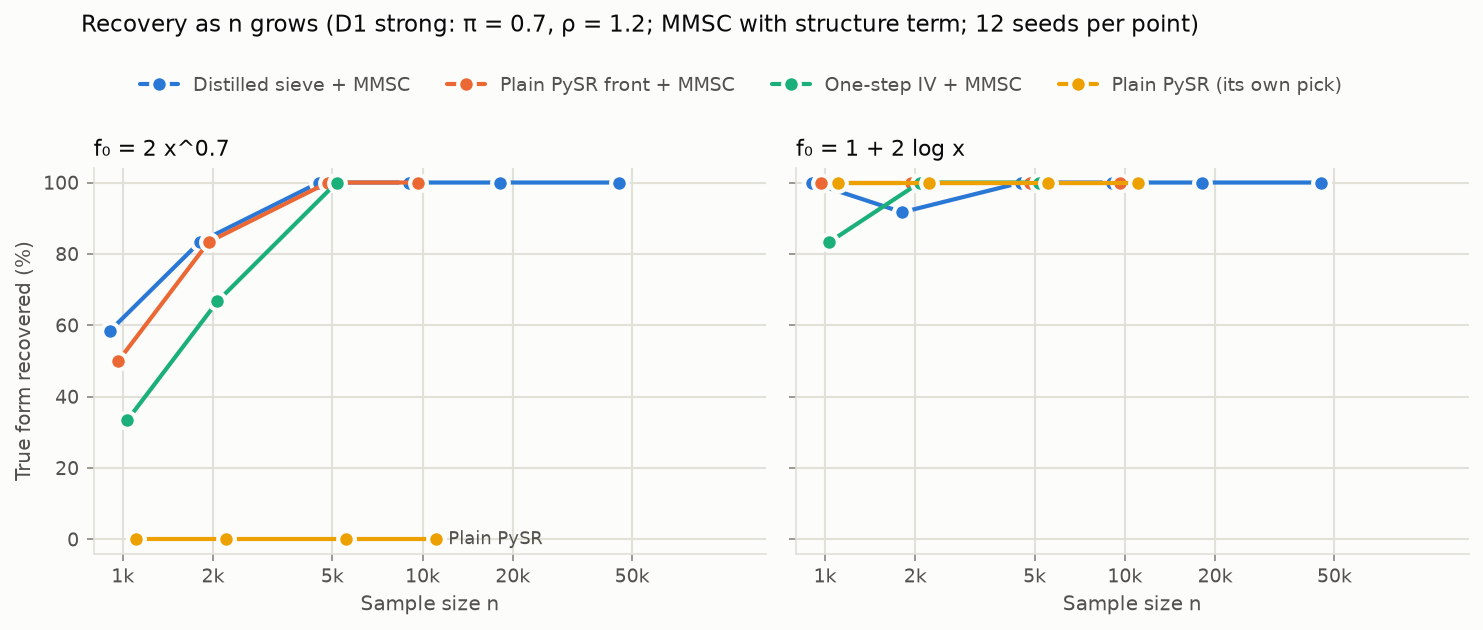
\includegraphics[width=\textwidth]{fig_nscale_light.png}
\caption{Recovery against sample size in the D1 strong setting ($\pi = 0.7$, $\rho = 1.2$), for the distilled, plain-PySR and one-step candidates scored by BIC + structure, and for plain PySR's own pick; 50 seeds per point at $n \le 5000$, 12 beyond.}
\label{fig:nscale}
\end{figure}

The instrument does its work when formulas are scored, not when they are generated. On the same runs (D1--D4), MMSC-BIC recovered the law from plain PySR's front about as often as from the IV-specific fronts: 52\%, against 47\% (one-step), 52\% (distilled) and 48\% (pooled). In the strong-endogeneity $n$-scaling cells, PySR's own pick recovered the power law in no run at any $n$ (50 seeds per cell up to $n = 5000$, 12 beyond), yet its front contained the true form in every run and the moment criterion selected it in 66--100\% of runs (Figure~\ref{fig:nscale}). Where PySR's own pick does get the form, its constants are biased: the log-law slope is 2.38--2.41 in D1, D2 and D4 against 2.00 with the moment criterion, and its in-sample errors are 5--16 times larger. IV-specific generators matter where endogeneity changes the shape of $\E[y \mid X]$: under simultaneity (D3) the plain front contains the true form in 25\% of runs, against 44--48\% for the one-step and distilled fronts. The cheap generators are also faster: over the full grid, whose samples reach $n = 50{,}000$, a median of 9 seconds per plain or distilled search against 61 for the one-step search (26 against 4 at $n = 2000$ in Section~\ref{sec:mc-first}).

A structure term is needed. BIC plus $0.5\,\ell_s\log m$ raised pooled recovery from 51\% to 60\% (Table~\ref{tab:rules}; 46 runs won, 8 lost; McNemar $p < 0.001$). In the $n$-scaling cells it gave 98--100\% recovery at $n = 5000$ (50 seeds) and 100\% from $n = 10{,}000$ for every generator. With BIC alone, recovery of $2x^{0.7}$ plateaus at 86--90\% at $n = 5000$ and 75--92\% from $10{,}000$ to $50{,}000$: the rest chose a near-duplicate such as $(xe^{x/\max(c, x)})^{0.7}$ or $x^{0.75}(xe^{-x} + 1.74)$, which has the same number of constants as the truth, differs from it only at small $x$, and is separated by its size, not by the moments. This is the case that falls under neither channel of \res{Theorem}{2} and that the per-node penalty resolves. The term costs recovery on the saturation law, whose true form $ax/(b + x)$ is long: pooled recovery in D1 fell from 42\% to 25\%; the templates of Section~\ref{sec:budget} more than repair that. HQIC (44\%), AIC (24\%) and the cross-fitted criterion (28\%) are worse than BIC; cross-fitting fails because over-parameterized formulas that contain the truth tie with it on held-out moments (\res{Theorem}{1}, Remark~4). Doubling $K$ changed nothing (16 runs won, 17 lost); kernel instruments were slightly better than splines (54\% against 51\%; 19 won, 6 lost; $p = 0.015$).

Distilled fronts select better than one-step fronts, and pooling does not help. Distilled fronts contain the true form more often than one-step fronts (74\% against 65\%) and hold fewer wrong formulas that outscore the truth under BIC (1.0 against 1.6 per run; at least one in 32\% against 44\% of runs). Pooling, a median of 28 candidates per run, raises coverage to 79\% but nearly triples these wrong formulas (2.9 per run), so recovery given coverage falls from 84\% to 72\% and the pooled set does not beat the distilled front alone. The library baseline's limit is coverage, not the IV logic: its Lasso path scored by the moment criterion recovers the log law in 100/100/92/75\% of runs in D1--D4 (against 28--52\% with cross-validated Lasso in the D1 and D2 cells of Section~\ref{sec:mc-baselines}), and given coverage it recovers 96\% of the time, but it contains the true form in only 35\% of runs because only the log law is in its library. Dropping \code{max} does not help: in paired comparisons no difference exceeded 3 runs ($p \ge 0.25$), and without \code{max} contrived winners use other operators.

Separation explains the selection failures, in a corrected form. The separation constant $\delta_L$ over all wrong trees was about zero in every cell and unrelated to recovery (Spearman 0.10), for two reasons: trees with more constants than $f_0$ approximate it arbitrarily well, and with a four-point instrument a tree with four constants can set the criterion to zero (\res{Proposition}{4}). The quantity that matters is the penalty-adjusted margin of~\eqref{eq:margin}, $\min_s[n\delta_s/\sigma_u^2 - (p_0 - p_s)\ln n]$ with the error variance $\sigma_u^2$ as the normalization $\sigma^2$ of~\eqref{eq:margin}, over wrong trees with $p_s \le p_0$, computed with the instruments the selection used on 20{,}000 noise-free draws, over the wrong formulas any run produced. Among runs whose candidates contained the true form it tracked recovery: Spearman 0.56 ($p < 0.001$) across 32 cells, 74\% recovery when the margin is positive and 23\% when it is not (Figure~\ref{fig:separation}). The margin is a worst case over the wrong formulas that were actually proposed, and the deviation terms of \res{Theorem}{2} explain why a small positive margin is not enough.

\begin{figure}[ht]
\centering
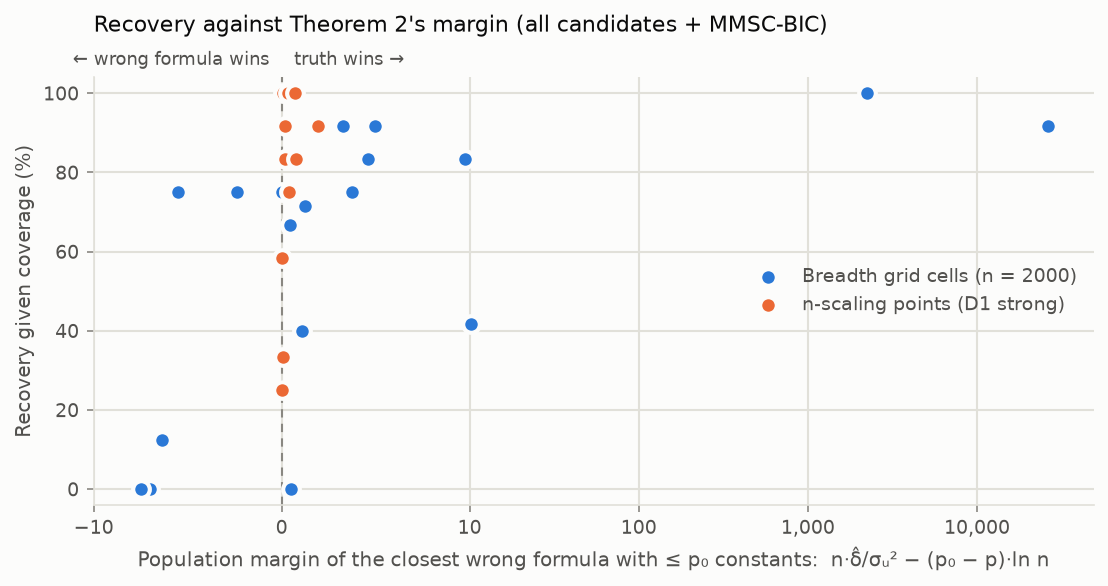
\includegraphics[width=\textwidth]{fig_separation_light.png}
\caption{Recovery given coverage against the penalty-adjusted separation margin, one point per cell of the breadth and $n$-scaling grids. Cells with a positive margin mostly recover the law; cells with a negative margin mostly do not.}
\label{fig:separation}
\end{figure}

The method fails in two places. The kink law was recovered in no pooled run, and no generator produced it in more than 33\% of runs; the saturation law appeared in 25--58\% of runs in D1--D4: search failures, taken up in Section~\ref{sec:budget}. Under the weak instrument (D5) recovery is 0--2\% for every law over 50 seeds; the selected formulas err by 0.3--1.0 sd in sample and 2.2--6.2 out of sample, and plain PySR's own pick is more accurate for two of the five laws in sample and four of five out of sample. The method should report weak identification there rather than a formula, and Section~\ref{sec:mc-ident} shows that it does. The control-function grid was inconclusive by design: with $\gamma = 0.45$ and $0.6$ control-function SR still never recovered the power law, but its log-law recovery rose to 83\% and 100\% because a larger $\gamma$ also increases the variance of $X$ given $Z$. On accuracy (D1--D4, pooled + structure), the median in-sample error is 0.040 against 0.129 for the sieve-2SLS curve; out of sample it is 0.074 when the form is recovered, 0.85 when it is not, and 0.76 for the sieve curve.

\subsection{Inference after selection}
\label{sec:mc-theory}

The remaining experiments test the theory on the saved fronts, with no new searches. The first tests \res{Theorem}{1(iii)}. For each run of the breadth grid at $n = 2000$, the law's own form and the formula selected by the pooled candidates with BIC + structure (when it has the true form) were estimated by two-step GMM on ten fresh samples and on the selection sample itself: 4{,}500 fits. Table~\ref{tab:inference} shows that on independent samples the intervals, the $J$ test and the AR sets are nominal, for the selected tree as for the oracle, and the standard errors are calibrated (the standard deviation of $\hat\theta - \theta_0$ across fresh samples is 0.84--1.00 times the mean reported standard error). On the selection sample, coverage of the constants drops to 83--90\% in D1--D3 (94\% with the discrete instrument): the post-selection distortion that splitting removes \citep{leebpotscher2005}. Under the weak instrument, Wald intervals for the oracle tree cover the constants 76\% of the time, the function at the median 68\% and the elasticity 64\%, and the $J$ test over-rejects, while the AR set at the true constants covers 97\%: AR inference survives weak identification of the constants, Wald inference does not. (A5)(a) held: every selected tree had a unique set of constants reproducing $f_0$.

\begin{table}[ht]
\centering\small
\caption{Inference after selection: coverage of nominal 95\% intervals and rejection rates of 5\% tests, 4{,}500 two-step GMM fits on the breadth-grid runs.}
\label{tab:inference}
\fittable{%
\begin{tabular}{@{}lccccc@{}}
\toprule
& Constants covered & $f$(median) & Elasticity & $J$ rejects & AR covers \\
\midrule
D1--D4, oracle, fresh samples & 93--95\% & 93--94\% & 92--96\% & 3--6\% & 93--97\% \\
D1--D4, selected tree, fresh samples & 92--98\% & 94--95\% & 92--94\% & 3--7\% & 93--97\% \\
D1--D4, selected tree, same sample & 83--94\% & 87--100\% & 88--96\% & 0--6\% & 94--97\% \\
D5 weak $Z$, true form, fresh samples & 76\% & 68\% & 64\% & 10\% & 97\% \\
\bottomrule
\end{tabular}}
\end{table}

\subsection{Candidates from one sample, selection on another}
\label{sec:mc-split}

This experiment tests \res{Corollary}{2.3} in the D1 strong setting, with the $n = 1000$ fronts and 12 seeds. When the same candidates are selected on five fresh samples of $n = 1000$ instead of the sample they were fitted to, the wrong candidates that outscore the truth fall from 1.92 to 1.37 per run (power law) and from 0.42 to 0.12 (log law), and recovery at equal selection size changes by $-2$ to $+25$ points across seven cells (median $+12$). But same-sample selection on the full $n = 2000$ with the structure term recovers more in all three BIC + structure cells (67\% against 47\%, 83\% against 72\%, 100\% against 92\%), because halving the sample halves the separation $n\delta_s$. Splitting is the right tool for inference, not for selection. The full table is in Appendix~\ref{app:tables}.

\subsection{The identification diagnostic}
\label{sec:mc-ident}

To test \res{Proposition}{5}, the report was run on every breadth-grid run, 630 after the 50-seed extension, with the pooled candidates and the BIC + structure selection on the run's own data ($\tau = 0.2$).

\begin{table}[ht]
\centering\small
\caption{The identification diagnostic on the 630 breadth-grid runs.}
\label{tab:ident}
\fittable{%
\begin{tabular}{@{}lcccc@{}}
\toprule
& Runs & Flagged (weakly identified or rejected) & Of which rejected & True form in $\Cc_\alpha$ \\
\midrule
D5 weak instrument, all runs & 250 & \textbf{100\%} & 16\% & 99\% \\
D1--D4, selection recovered the form & 257 & 4\% & 2\% & 99\% \\
D1--D4, statistical failure & 43 & 30\% & 7\% & 100\% \\
D1--D4, search failure & 80 & 54\% & 14\% & -- \\
\bottomrule
\end{tabular}}
\end{table}

Table~\ref{tab:ident} shows: coverage, \res{Proposition}{5}(a), across the 404 runs in which the true form was a candidate it is in the confidence set in 400 (99\%; nominal $\ge 95\%$). The weak instrument is always caught: in D5 the median first-stage $F$ is 3, 88\% of the candidates are not rejected, and the farthest member of the set differs from the selected formula by 0.8 sd (median); 84\% of the runs are reported ``weakly identified'' with the formulas the data also allow listed, and 16\% ``rejected''. False alarms are 4\% of the strong-instrument runs whose selection was right, the rate the 5\% AR level implies (at $\tau = 0.1$ it would be 14\%, with 58\% of the statistical failures caught instead of 30\%; Table~\ref{tab:tau}). Statistical failures, \res{Proposition}{5}(b): the true form was in the confidence set in all 43, and the diagnostic reports it as a different formula in 30\%; the other 70\% are near-duplicates within 0.2 sd of the truth, where the function is identified and only the tree is not minimal. Search failures: 54\% flagged, because the candidates that fit the moments disagree among themselves; the rest, mostly D3 with the kink and saturation laws, pass as ``identified'' because the wrong formula fits the moments and the other candidates agree with it, a case no diagnostic computed from the candidates can detect. With the discrete instrument (D4), 35\% of runs are ``weakly identified'' despite $F \approx 640$: with $K = 4$ moments the S test has little power, and the set contains formulas up to 0.13 sd away, \res{Proposition}{4} in the data.

\subsection{Discrete instruments}
\label{sec:mc-discrete}

\res{Proposition}{4} is visible in design D4 ($J = 4$), where the criterion has $K = 4$. On 20{,}000 noise-free draws, the wrong four-constant formula $c_0 + c_1\sqrt x + c_2x + c_3x^2$ fitted to the moments sets the criterion to $10^{-33}$--$10^{-32}$ for the power, kink and saturation laws while missing $f_0$ by 0.12, 0.15 and 0.42 standard deviations: \res{Proposition}{4}(a). For the log law the solution of the four moment equations lies outside the constant bound $\abs{c} \le 10$, so the bound, not the moments, keeps the criterion positive. Under D1's continuous instrument the same formula is separated from each law.

\section{Applications}
\label{sec:apps}

\subsection{Simulated economic environments}
\label{sec:apps-sim}

Two environments extend the grid to shapes that were not in it, with 20 seeds per law at $n = 2000$, candidates from plain PySR, distillation and the library path pooled, and selection by BIC + structure.

\emph{Demand with a cost shifter} (design D6, the mirror image of D3): quantity $q = f_0(p) + u$ is a decreasing demand curve, the supply equation $q = \kappa\log p + \gamma Z + e$ is shifted by a cost shifter $Z$, and the price is set by equilibrium. Demand laws: constant elasticity $3p^{-0.5}$, log-linear $6 - 1.5\log p$ (in the library), and hyperbolic $6/(1 + p)$.

\emph{Backward-bending labour supply}: hours $h = f_0(w) + u$, the wage endogenous because unobserved taste for work is correlated with productivity, the instrument an exogenous wage shifter; design D1 with $\pi = 0.5$ and the laws $8we^{-0.5w}$ (a hump) and $5 + 2\log w - 0.6(\log w)^2$ (the textbook quadratic in logs); and a control with $\pi = 1$ and a flatter quadratic, $5 + 0.5\log w - 0.6(\log w)^2$, whose peak lies near the median wage.

\begin{table}[ht]
\centering\footnotesize
\setlength{\tabcolsep}{3.5pt}
\caption{Simulated economic environments: 20 seeds per law, $n = 2000$. ``Plain'' is PySR's own pick (recovered / error); ``Pooled'' pools plain PySR, distillation and the library path; errors in units of sd$(f_0)$; elasticities at the median.}
\label{tab:environments}
\fittable{%
\begin{tabular}{@{}llcccccc@{}}
\toprule
Environment & Law & \makecell{Plain:\\recov.\ / error} & \makecell{Pooled\\+ BIC} & \makecell{Pooled + BIC\\+ structure} & \makecell{Error:\\sel.\ / oracle} & \makecell{Elasticity:\\truth / sel.} & $F$ \\
\midrule
Demand, D6 & $3p^{-0.5}$ & 0\% / 0.43 & 95\% & \textbf{100\%} & 0.029 / 0.029 & $-0.50$ / $-0.49$ & 332 \\
Demand, D6 & $6 - 1.5\log p$ & 0\% / 0.33 & 90\% & \textbf{100\%} & 0.024 / 0.024 & $-0.62$ / $-0.62$ & 338 \\
Demand, D6 & $6/(1 + p)$ & 0\% / 0.57 & 65\% & \textbf{70\%} & 0.041 / 0.025 & $-0.78$ / $-0.77$ & 330 \\
Labour, $\pi = 0.5$ & $8we^{-0.5w}$ & 0\% / 0.42 & 60\% & \textbf{75\%} & 0.040 / 0.033 & 0.50 / 0.49 & 40 \\
Labour, $\pi = 0.5$ & $5 + 2\log w - 0.6(\log w)^2$ & 0\% / 0.30 & 10\% & \textbf{0\%} & 0.347 / 0.051 & 0.40 / 0.29 & 40 \\
Labour, $\pi = 1$ (control) & $8we^{-0.5w}$ & 60\% / 0.21 & 75\% & \textbf{75\%} & 0.027 / 0.025 & 0.50 / 0.51 & 161 \\
Labour, $\pi = 1$ (control) & $5 + 0.5\log w - 0.6(\log w)^2$ & 10\% / 0.37 & 20\% & \textbf{20\%} & 0.190 / 0.032 & 0.10 / 0.10 & 161 \\
\bottomrule
\end{tabular}}
\end{table}

Demand curves are recovered (Table~\ref{tab:environments}). With a cost shifter, the constant-elasticity and log-linear demand curves are recovered in every run, with the oracle's error and the right price elasticity; plain PySR never recovers them, its picks carrying the simultaneity bias (errors 0.3--0.6 sd). The hyperbolic demand is recovered in 70\% of runs, the misses being near-duplicates such as $3.3p^{-0.74}$ with the elasticity still right. Backward-bending labour supply exposes a limit: with $\pi = 0.5$ only 7\% of wages lie past the peak of the quadratic-in-logs law, and the law is never recovered; in 7 of the 9 runs where it was a candidate a simpler wrong formula beat it (channel (I) of \res{Theorem}{2}), and the selected formulas are worse in sample than plain PySR's. The hump law, whose peak sits inside the data, is recovered in 75\% of runs with near-oracle error. The control shows what identification needs: with $\pi = 1$ and the quadratic's peak near the median wage, recovery rises only to 20\%, and now every miss is a search failure, since the three-constant form was a candidate in just 20\% of runs and, whenever it was, it was selected. For these shapes the binding constraint is the search's coverage of three-constant forms, not selection; Section~\ref{sec:budget} supplies the form as a template and recovery rises to 75\%. The diagnostic says ``identified'' in every demand run, and ``weakly identified'' in 85--95\% of the hump runs even where the form was recovered: candidates 0.2--0.4 sd away fit the moments as well as the truth, because a bump is a feature that the smoothing of $\E[\cdot \mid Z]$ nearly erases. The recovered hump is correct but not pinned down by the data, and the method says so.

\subsection{Engel curves}
\label{sec:engel}

The primary application has a continuous instrument and a formula-shaped known answer. The data are the public Family Expenditure Survey 1995 sample of \citet{bck2007}, 1{,}655 married couples with an employed head aged 25--55 (628 without children, 1{,}027 with), shipped as the \code{Engel95} data frame of the R package \code{np}: seven budget shares, log total expenditure, the head's log earnings, and a children indicator. Each share is regressed on log total expenditure, instrumented by the head's log earnings ($K = 9$--$12$ spline instruments; first-stage $F$ = 31--59), in the full sample and in the two subsamples. Candidates come from plain PySR, distillation, the library path and the templates, pooled; selection by BIC + structure; then the identification report, and the S tests of the Working--Leser form (share linear in log expenditure) and of the quadratic form, with an AR interval for the quadratic term. The known answers are that food is Working--Leser and that some goods need a quadratic term \citep{bankslewbel1997}. On synthetic FES-like data with a planted Working--Leser share, the same pipeline recovers $0.452 - 0.060\log x$ from $0.45 - 0.06\log x$ and reports ``identified''.

\begin{table}[ht]
\centering\footnotesize
\setlength{\tabcolsep}{3.5pt}
\caption{Engel curves on the FES 1995 sample: the selected formula in the full sample, the verdict in the three samples (all couples / no children / with children), whether the Working--Leser form is rejected, and whether the quadratic term's AR interval excludes zero. ``Weak'' is ``weakly identified'', ``rej.'' is ``rejected''.}
\label{tab:engel}
\fittable{%
\begin{tabular}{@{}llllll@{}}
\toprule
Share & Selected, all couples & Shape & Verdict & \makecell[l]{Working--Leser\\rejected} & \makecell[l]{Quadratic AR\\excludes 0} \\
\midrule
food & $0.747^x$ (share $\propto$ expenditure$^{-0.29}$) & decreasing & weak / weak / weak & no / no / no & no / no / no \\
catering & constant 0.080 & flat & weak / weak / weak & no / no / no & no / no / no \\
alcohol & $0.19 - 0.025\log x$ (a template) & decreasing & weak / weak / weak & no / no / no & no / no / no \\
fuel & $(\log x)^{-5.3}$ & decreasing & weak / weak / weak & no / no / at the margin & no / no / at the margin \\
motor & $0.693^x$; in the set: $0.025/\max(0.17, x - 5.74)$ & decreasing & \textbf{rej.} / weak / \textbf{rej.} & \textbf{yes} / no / \textbf{yes} & \textbf{yes} / \textbf{yes} / \textbf{yes} \\
fares & constant 0.015; in the set: $0.0028x$ & flat & \textbf{rej.} / weak / weak & no / no / no & no / no / no \\
leisure & $0.00051e^x$ (share $\propto$ expenditure) & increasing & weak / weak / weak & no / no / no & no / no / no \\
\bottomrule
\end{tabular}}
\end{table}

The known answers hold (Table~\ref{tab:engel}). The food share is compatible with Working--Leser in all three samples: the linear-in-log-expenditure form is never rejected and the quadratic term's AR interval always contains zero. The motor share needs a quadratic term: its AR interval excludes zero in all three samples and the Working--Leser form is rejected in two, the case \citet{bankslewbel1997} make for some goods. Fuel sits at the margin in the with-children sample (18.4 against a critical value of 18.3; AR interval $[0.000, 0.084]$). Leisure is a luxury (increasing), food and fuel necessities (decreasing); catering and fares are flat within the data's power. No share is ``identified'': with 628--1{,}655 households and shares whose noise dwarfs their structural variation, 24--40 candidates per share pass the S test, up to 0.25--2.8 sd of the selected curve apart, and the report lists them instead of claiming one formula. The selection fails its own S test three times (motor twice, fares once); the pick restricted to the confidence set is then reported, a kinked hyperbola for motor and a line through the origin for fares. Plain PySR's own pick coincides with the IV selection for food, fuel and motor in the full sample: on these data the conditional-mean and structural shapes are close in the bulk of the sample, so the instrument's work shows in the tests and the set, not in the pick. The templates changed one pick (alcohol, all couples: the Working--Leser template replaced a quadratic in the level of log expenditure). The 21 runs took about 15 minutes.

\subsection{Angrist--Krueger as a stress test}
\label{sec:ak}

\citet{angristkrueger1991} instrument schooling by quarter of birth. The instruments are weak \citep{boundjaegerbaker1995}, discrete, and shift schooling only near the compulsory-schooling margin, so they cannot identify a functional form over the whole range; the test of the method is whether it says so. The data are the public \emph{Mastering 'Metrics} extract: 329{,}509 men born 1930--39, log weekly wage demeaned within birth year, schooling as the endogenous regressor. The replication is exact: with the 30 within-cohort quarter-of-birth contrasts (Angrist and Krueger's Table V) the first-stage $F$ is 4.9 (Bound, Jaeger and Baker report 4.7--4.9), the OLS return 0.071 and the 2SLS return 0.089 (Angrist and Krueger: 0.071 and 0.089); with the three overall contrasts, $F = 34$ and 2SLS gives 0.103. Both instrument sets select $\log(0.075(s + 1))$, a concave return profile (0.10 per year at 9 years of schooling, 0.07 at 13, 0.06 at 17), which is also plain PySR's own pick: the moments do not move the formula away from the conditional-mean shape. The diagnostic says ``weakly identified'' with both sets: every other candidate survives its S test (25 of 25 with 30 instruments; 23 of 23 with 3), the farthest 1.1--1.3 sd from the selected formula. The identification-robust AR interval for the linear return is $[-0.01, 0.44]$ against the Wald interval $[0.06, 0.16]$ with 30 instruments, and $[-0.01, 0.26]$ against $[0.03, 0.18]$ with 3: two to five times wider, and including zero. With 3 instruments ($K = 4$) any formula with four constants fits the moments exactly (\res{Proposition}{4}); with 30, the compulsory-schooling variation is too small to tell shapes apart. A confident formula would have been wrong here, and the method does not give one. The sieve-2SLS curve shows the instability of unrestricted NPIV: with 3 instruments it moves by $-1.0$ log points between 8 and 12 years of schooling and by $+2.5$ between 12 and 16.

\section{Search budget and templates}
\label{sec:budget}

In the cells where the search rarely proposed the law, D1 and D3 with the kink and saturation laws and the two quadratic labour-supply laws, coverage rather than selection was the binding constraint. This section asks whether a larger search budget or a fixed library of templates repairs that. Four arms on the same data and seeds (88 runs, 352 analyses; the searches are new and the one-step front is not used, so the base rates differ from those of Section~\ref{sec:mc}): the \emph{base} budget (40 iterations, 31 populations, size $\le 15$); base \emph{+ templates} (the eleven shapes of Section~\ref{sec:generators}, scored like any candidate); a \emph{large} budget (200 iterations, 40 populations, size $\le 25$, two restarts pooled: about eight times the compute, 2--2.7 minutes per run instead of 6--19 seconds); and large + templates. Plain PySR and distillation only, plus the library path; selection by BIC + structure.

\begin{table}[ht]
\centering\footnotesize
\setlength{\tabcolsep}{4pt}
\caption{Coverage $\to$ recovery by cell and arm (pooled candidates; coverage means some candidate has the true form).}
\label{tab:budget}
\fittable{%
\begin{tabular}{@{}llcccc@{}}
\toprule
Cell & Law & Base & \makecell{Base +\\templates} & Large & \makecell{Large +\\templates} \\
\midrule
D1 & $x - 0.8\max(x - 1.5, 0)$ & 0\% $\to$ 0\% & 100\% $\to$ 0\% & 8\% $\to$ 0\% & 100\% $\to$ 0\% \\
D1 & $3x/(1 + x)$ & 50\% $\to$ 42\% & 100\% $\to$ \textbf{67\%} & 42\% $\to$ 17\% & 100\% $\to$ 50\% \\
D3 & $x - 0.8\max(x - 1.5, 0)$ & 0\% $\to$ 0\% & 100\% $\to$ 0\% & 0\% $\to$ 0\% & 100\% $\to$ 0\% \\
D3 & $3x/(1 + x)$ & 25\% $\to$ 0\% & 100\% $\to$ 8\% & 42\% $\to$ 17\% & 100\% $\to$ 8\% \\
Labour, $\pi = 0.5$ & $5 + 2\log w - 0.6(\log w)^2$ & 45\% $\to$ 0\% & 100\% $\to$ 0\% & 90\% $\to$ 5\% & 100\% $\to$ 0\% \\
Labour, $\pi = 1$ & $5 + 0.5\log w - 0.6(\log w)^2$ & 20\% $\to$ 20\% & 100\% $\to$ \textbf{75\%} & 95\% $\to$ 60\% & 100\% $\to$ 60\% \\
\midrule
All 88 runs & & 25\% $\to$ 10\% & 100\% $\to$ \textbf{27\%} & 55\% $\to$ 19\% & 100\% $\to$ 22\% \\
Recovery given coverage & & 41\% & 27\% & 35\% & 22\% \\
Candidates per run (median) & & 24--30 & 34--40 & 57--68 & 68--80 \\
Beaters per run (wrong formulas that outscore the truth) & & 2.9 & 3.8 & 4.8 & 5.8 \\
\bottomrule
\end{tabular}}
\end{table}

Paired on the same data (Table~\ref{tab:budget}): large against base, coverage $+33/-7$ runs ($p < 0.001$), recovery $+13/-5$ ($p = 0.10$); base + templates against base, recovery $+15/-0$ ($p < 0.001$); large + templates against large, $+4/-2$ ($p = 0.69$). Four findings.

\begin{enumerate}
\item \emph{A larger search budget buys coverage, not recovery.} Eight times the compute raised coverage from 25\% to 55\% of runs and found the three-constant quadratic labour law in 90--95\% of runs instead of 20--45\%. Recovery rose only from 10\% to 19\%, not significantly, because the extra candidates bring extra wrong formulas that outscore the truth, 4.8 per run instead of 2.9, and recovery given coverage fell from 41\% to 35\%. In the D1 saturation cell the large budget \emph{lost} four runs the base budget had recovered. This is channel (II) of \res{Theorem}{2} and the pooling result of Section~\ref{sec:mc-grid} again: the size of the candidate pool is a cost in itself.
\item \emph{Templates buy coverage for free, and recovery where the moments separate the law.} With the true form always a candidate, the quadratic labour law at $\pi = 1$ went from 20\% to 75\% ($p = 0.001$; the template or an equivalent rearrangement is the pick in 15 of 20 runs) and the saturation law in D1 from 42\% to 67\%. Base + templates is the best arm overall (27\%), at the base cost. Adding the large budget's candidates to the templates makes things worse (22\%): more candidates, more beaters.
\item \emph{Where nothing helps, the limit is separation.} The kink law is never recovered: even with the template in the pool, a one- or two-constant formula such as $x^{0.54}$ beats the three-constant kink under BIC + structure, because the moments barely distinguish them (the kink pays about 22 more in penalty and gains less than that in $J$); in D3, where only 6\% of the regressor's mass lies past the kink, the identity $x$ wins. The quadratic labour law at $\pi = 0.5$ is found by the large budget in 90\% of runs and selected in 5\%: only 7\% of wages lie past its peak. A threshold or a bend has to be inside the data and inside the instrument's reach.
\item \emph{The method to present:} cheap generators (plain PySR and distillation at the base budget, and the library path) plus the template library, selection by BIC + structure, then the identification diagnostic. A larger free search is optional; if used, its candidates should be pruned before pooling, not added wholesale.
\end{enumerate}

\section{Conclusion}
\label{sec:limits}

This paper has asked whether a symbolic-regression search can recover a structural equation when the regressors are endogenous, and has answered by moving the instrument from the generation of candidate formulas to their scoring. Candidates may come from any cheap generator, a squared-error search, a distilled nonparametric IV curve, a sparse library path or a list of textbook shapes; each is refitted by GMM on sieve instruments, the formula is selected by a GMM model-selection criterion with a per-node structure penalty, and an Anderson--Rubin confidence set over formulas reports whether the data identify the result. The approach treats symbolic regression and instrumental variables as complements: the search supplies the functional forms that econometrics would otherwise have to assume, and the moment conditions supply the identification that the search lacks.

The theoretical results characterize when this works. The selection rule is consistent for any generator whose candidates contain the true form, the constants of the selected formula converge at the parametric rate, and split-sample GMM inference on it is valid (\res{Theorem}{1}). The finite-sample bound of \res{Theorem}{2} isolates the two channels through which selection fails, a wrong formula that the moments barely separate from the truth and a longer formula that fits the moment noise, and shows that the structure penalty is what controls the second channel uniformly in the formula size. \res{Proposition}{5} establishes that the formula confidence set covers the true form without any rank condition, which is what allows the method to report weak identification rather than a confident formula, and \res{Proposition}{4} shows that a $J$-point instrument cannot exclude formulas with $J$ or more constants, so that discrete instruments bound the complexity the moments can discipline.

The Monte Carlo evidence is consistent with these results. Under confounding and a heteroskedastic first stage the method recovers the log, power and two-regressor laws in 92--100\% of runs, and in 60--92\% under simultaneity and a discrete instrument; in the strong-endogeneity setting its recovery of the log and power laws reaches 98--100\% from $n = 5000$, whereas the squared-error search never recovers the power law under strong endogeneity and, where it finds the log form, carries a slope bias equal to $\rho/(1 + \pi^2)$ to two decimals. The contribution of the instrument is concentrated in the scoring step: candidates from a plain search, from a distilled sieve-2SLS curve or from a library of economic templates, selected by the moment criterion, perform as well as or better than a search run on the moment criterion itself. Under a weak instrument recovery falls to 0--2\% and the diagnostic flags every run, at a 4\% false-alarm rate under strong instruments. On the 1995 Family Expenditure Survey the method reproduces the Working--Leser food share and the quadratic motor share of the Engel-curve literature, and on the quarter-of-birth instruments of \citet{angristkrueger1991} it reports weak identification rather than a formula.

Two limitations of the method are documented in Sections~\ref{sec:mc}--\ref{sec:budget} and not resolved. A threshold law whose kink the instruments barely move is not recovered at $n = 2000$, because a simpler formula fits the moments equally well, and a backward-bending labour supply whose bend lies at the edge of the data is found by a large search in 90\% of runs but selected in 5\%, for the same reason. Both are failures of identification within the formula class rather than of the selection rule, and the diagnostic flags only part of them, since a wrong formula that fits the moments is, by the data's lights, identified. A larger search budget does not help in either case; instruments whose support extends through the kink or the bend, or substantially larger samples, would.

Several questions remain open. Rates of convergence for a growing formula size reduce, by \res{Proposition}{3.3}, to a modulus of continuity on the formula sieve; because the sieve less $f_0$ is not a linear space, the modulus can fall below any quadratic, and bounding it for specific sieves, free-knot splines first, is the natural next step. \res{Theorem}{3(b)} is stated on a compact support; the lognormal designs require a growth envelope in place of the Lipschitz ball, approximants that respect it (clipping with \code{max} and \code{min} does, at the cost of nodes), and a concentration inequality under an unbounded envelope, each of which appears routine and none of which is written out. \res{Theorem}{2} covers the sieve criterion with any fixed positive definite weight; the exact kernel criterion is a degenerate V-statistic at the truth and requires concentration for degenerate U-processes, and an estimated efficient weight enters through \res{Proposition}{2.4} and requires a concentration bound for the weight estimate. For discrete instruments, whether a wrong tree with fewer than $J$ constants is generically identified is a transversality question, stated as \res{Conjecture}{4(c)} in Appendix~\ref{app:prop4}, whose regular-value hypothesis we cannot verify in general. The consistency result is pointwise in the data-generating process; a uniform version over designs whose separation is bounded below would follow from \res{Theorem}{2} with explicit sample sizes. Finally, the additive error excludes random coefficients, and the IV quantile model of \citet{chernozhukovhansen2005} is the natural route to a non-separable extension.

For applied work the results suggest a simple protocol. Candidates should be generated cheaply and include templates for the shapes that economic theory names; the formula should be refitted and selected by the moment criterion with the BIC penalty per constant and the structure term per node; the number of constants should be capped at $J - 1$ when the instrument takes $J$ values; inference should use a split sample; and the identification diagnostic should be reported in every case, since it is the method's answer where the data do not identify a formula. A larger search is optional, and its candidates should be pruned before they are pooled. The code, the run records and a replication guide accompany the paper.


\section*{Replication}
\addcontentsline{toc}{section}{Replication}
Every number in this paper is produced by the scripts in the repository \url{https://github.com/manuzrpEd/IV_SymbolicRegression} from the run records committed there; the file \code{REPLICATION.md} gives the exact software versions (Python 3.12, PySR 2.6.0, SymbolicRegression.jl 2.5.1, Julia 1.11), the data provenance with checksums, the measured runtime of every step (about 40 hours of compute on a four-core laptop; Table~\ref{tab:compute}), the seeds, and a map from each table and figure to the script and output file that produce it. The searches themselves are stochastic and reproduce the reported rates in distribution; everything downstream of the saved Pareto fronts is deterministic and reproduces the committed files exactly. The two application data sets are public: the \code{Engel95} data frame of the R package \code{np} \citep{bck2007} and the Angrist--Krueger extract distributed with \emph{Mastering 'Metrics}; neither is redistributed. No confidential data were used.

\section*{Acknowledgements}
\addcontentsline{toc}{section}{Acknowledgements}
Claude (Anthropic) assisted with this project throughout: it implemented the code under the author's direction, ran the experiments, derived and checked the proofs, and drafted the text; two fresh-context instances read the proofs as referees before this draft. The author designed the study, directed every step, and is responsible for all content and any errors. No funding was received.

\bibliography{references}

\appendix
\section{Proofs}
\label{app:proofs}

Throughout, $P_n$ denotes the empirical measure and $(P_n - P)[h] = n^{-1}\sum_ih(W_i) - \E h(W)$.

\subsection{Lemma 1}

\begin{proof}
(a) If $\theta_k \to \theta$ in $\Theta_s$, then $f_s(x;\theta_k) \to f_s(x;\theta)$ for every $x$, and $\abs{f_s(x;\theta_k) - f_s(x;\theta)}^2 \le 4F(x)^2$. Dominated convergence gives $L^2$ convergence. A continuous image of a compact set is compact, and a finite union of compact sets is compact.

(b) $\theta \mapsto \norm{T(f_s(\cdot;\theta) - f_0)}^2$ is continuous, by (a) and $\norm{T} \le 1$. It is positive on $\Theta_s$ by (A2), because a wrong tree never equals $f_0$. A positive continuous function on a compact set has a positive minimum.

(c) The set $\{f \in \Fc_L : \norm{f - f_0} \ge \varepsilon\}$ is closed in the compact $\Fc_L$, hence compact. The map $f \mapsto \norm{T(f - f_0)}^2$ is continuous, and by (A2) it is positive there.
\end{proof}

\subsection{Lemma 2}

\begin{proof}
\emph{(a), (C2).} The uniform law of large numbers \citep[Lemma 2.4]{neweymcfadden1994} applies to $\theta \mapsto b(z)(y - f_s(x;\theta))$ on each compact $\Theta_s$: the map is continuous, with integrable envelope $\norm{b(z)}(\abs{y} + F(x))$ (integrable by Cauchy--Schwarz). There are finitely many trees, and $\hat W \to_p W$.

\emph{(a), (C3).} $\sqrt n\,\hat g(f_0) = n^{-1/2}\sum_ib(Z_i)u_i$ has mean zero, because $\E[bu] = \E[b\,\E(u \mid Z)] = 0$. Its second moment is $\E[\norm{b}^2u^2] < \infty$, so it is $O_p(1)$ by Chebyshev's inequality.

\emph{(a), (C1).} $Q(f) = 0$ if and only if $g(f) = 0$, if and only if $\Pi_KT(f_0 - f) = 0$. Continuity follows from $\norm{g(f) - g(f')} \le (\E\norm{b}^2)^{1/2}\norm{f - f'}$.

\emph{(b), (C2).} Write $Q_n(f) = \norm{n^{-1}\sum_ir_i\varphi(Z_i)}_{\Hc}^2$ with $\varphi(z) = k(z, \cdot)$ and $\norm{\varphi(z)}_{\Hc} \le \sqrt{\bar\kappa}$. The same uniform-law argument works in the separable Hilbert space $\Hc$, using Mourier's strong law at the grid points.

\emph{(b), (C3).} $\E\norm{n^{-1/2}\sum_iu_i\varphi(Z_i)}_{\Hc}^2 = \E[u^2k(Z,Z)] \le \bar\kappa\E[u^2]$; the cross terms vanish because $\E[u\varphi(Z)] = 0$.

\emph{(b), (C1).} $Q(f) = \norm{\E[T(f_0 - f)(Z)\varphi(Z)]}_{\Hc}^2$. Continuity: $\norm{\E[h\varphi]}_{\Hc} \le \sqrt{\bar\kappa}\norm{h}$ and $\norm{T} \le 1$. For an integrally strictly positive definite kernel, $\norm{\E[h(Z)\varphi(Z)]}_{\Hc} = 0$ only if the finite signed measure $h\,dP_Z$ vanishes, i.e.\ $h = 0$ almost surely \citep{zhang2020,muandet2020}.
\end{proof}

\subsection{Theorem 1, Corollary 1.1 and Theorem 1(iii)}

\begin{proof}[Proof of \res{Theorem}{1}]
\emph{Setup.} Let $R_n := \sup_{f \in \Fc_L}\abs{Q_n(f) - Q(f)} = o_p(1)$, by (C2). Let $E_n$ be the coverage event. On $E_n$, pick $s^* \in \hat\Sc \cap \Sc_0$ (for (ii), in $\Sc_0^{\min}$) and $\theta^* \in \Theta_{s^*}^0$. Then $\hat Q_{s^*} \le Q_n(f_0)$, so
\begin{equation}
\crit_n(s^*) \le \frac{nQ_n(f_0)}{\hat\sigma^2} + \pen_n(s^*) = O_p(1) + O(\kappa_n).
\label{eq:crit-star}
\end{equation}

\emph{(i).} Because $\hat s$ minimizes $\crit_n$ over $\hat\Sc$ and penalties are nonnegative, $n\hat Q_{\hat s}/\hat\sigma^2 \le \crit_n(s^*)$. Then $\hat Q_{\hat s} \le \hat\sigma^2\crit_n(s^*)/n = o_p(1)$ by~\eqref{eq:crit-star} and $\kappa_n/n \to 0$, hence $Q(\hat f) \le \hat Q_{\hat s} + R_n = o_p(1)$. Fix $\varepsilon > 0$. By (C1) and \res{Lemma}{1}(a), $\eta(\varepsilon) := \inf\{Q(f) : f \in \Fc_L,\ \norm{f - f_0} \ge \varepsilon\} > 0$, the infimum of a positive continuous function over a compact set. So $P(\norm{\hat f - f_0} \ge \varepsilon) \le P(Q(\hat f) \ge \eta(\varepsilon)) + P(E_n^c) \to 0$.

\emph{(ii), wrong trees.} For a wrong $s$, $\delta_s^Q := \min_\theta Q(f_s(\cdot;\theta)) > 0$, by (C1) and compactness. On $E_n$, $\crit_n(s) \ge n\hat Q_s/\hat\sigma^2 \ge n(\delta_s^Q - R_n)/\hat\sigma^2$, which exceeds $\crit_n(s^*) = O_p(\kappa_n) = o_p(n)$ with probability tending to one. There are finitely many wrong trees, so $P(\hat s \notin \Sc_0) \to 0$.

\emph{(ii), over-parameterized true trees.} For $s \in \Sc_0$ with $p_s > p_0$, since $\hat Q_s \ge 0$,
\begin{align*}
\crit_n(s) - \crit_n(s^*) &\ge (p_s - p_0)\kappa_n + w(\ell_s - \ell_{s^*})\log m - \frac{nQ_n(f_0)}{\hat\sigma^2} \\
&\ge \kappa_n - wL\log m - O_p(1) \to \infty.
\end{align*}
So $P(\hat s \in \Sc_0,\ p_{\hat s} > p_0) \to 0$. Every tree outside $\Sc_0^{\min}$ is wrong or over-parameterized, there are finitely many, and each loses to $s^*$ with probability tending to one; therefore $P(\hat s \in \Sc_0^{\min}) \to 1$.
\end{proof}

\begin{proof}[Proof of \res{Corollary}{1.1}]
For a fixed $s \in \Sc_0^{\min}$, $\hat\theta_s$ is a GMM estimator (first step, or the two-step one) of a correctly specified moment model whose population moment vanishes exactly on the finite set $\Theta_s^0$, by (A2$_K$) and (A5)(a). Consistency to that set, $\dist(\hat\theta_s, \Theta_s^0) \to_p 0$, follows from the uniform law of \res{Lemma}{2}(a) and compactness as in \citet[Theorem 2.1]{neweymcfadden1994}; with probability tending to one $\hat\theta_s$ then lies in a neighbourhood of a single zero $\theta_{0s}$, on which the moment model is identified, and the local argument of their Theorem~3.4, with the regularity (A5)(b)--(d), gives $\sqrt n(\hat\theta_s - \theta_{0s}) = O_p(1)$. Then, for any $M$,
\[
P\bigl(\sqrt n\norm{\hat\theta_{\hat s} - \theta_{0\hat s}} > M\bigr) \le \sum_{s \in \Sc_0^{\min}}P\bigl(\sqrt n\norm{\hat\theta_s - \theta_{0s}} > M\bigr) + P(\hat s \notin \Sc_0^{\min}),
\]
which is small for $M$ and then $n$ large. The function bound follows from the Lipschitz property.
\end{proof}

\begin{proof}[Proof of \res{Theorem}{1(iii)}]
\emph{Fixed tree.} Fix $s \in \Sc_0^{\min}$. On $B$, $\tilde\theta(s)$ is the efficient GMM estimator of a fixed, correctly specified moment model. (A2$_K$) and (A5)(a) give identification up to the finite set $\Theta_s^0$ of isolated zeros, and the asymptotics are those of the zero nearest $\tilde\theta(s)$, as in the proof of \res{Corollary}{1.1}. Normality and the $J$ limit are then \citet{hansen1982} and \citet[Theorems 2.6 and 3.4]{neweymcfadden1994}; the consistency of $\hat\Omega$ and $\hat V$ uses $\E[\norm{b}^2\sup_\theta(y - f_s(X;\theta))^2] < \infty$, which \res{Lemma}{2}(a)'s setting provides.

\emph{Selected tree.} $\hat s$ is a function of $A$, and $A$ is independent of $B$ because the split does not depend on the data. So for any bounded continuous $\phi$, with $S_B(s)$ the studentized statistic for tree $s$,
\[
\bigl\lvert\E\phi(S_B(\hat s)) - \E\phi(N)\bigr\rvert \le \sum_{s \in \Sc_0^{\min}}P(\hat s = s)\bigl\lvert\E\phi(S_B(s)) - \E\phi(N)\bigr\rvert + 2\norm{\phi}_\infty P(\hat s \notin \Sc_0^{\min}) \to 0.
\]

\emph{Other statistics.} The same argument covers $J_B$ and $\AR_B$. The AR limit uses only the CLT for $\sqrt{n_B}\,\bar u_B$ and $\hat\Omega_B \to_p \Omega$.
\end{proof}

\subsection{Proposition 5 and the two guards}
\label{app:prop5}

\begin{proof}
(a) At $(s_0, \theta_0)$ the residuals are $u_i$, so $\hat g(s_0,\theta_0) = \bar u := n^{-1}\sum_ib_iu_i$ and $\hat\Omega_{s_0}(\theta_0) = n^{-1}\sum_ib_ib_i'u_i^2 \to_p \Omega$ by the law of large numbers. By (A1), $\E[bu] = 0$, and $\sqrt n\,\bar u \to_d N(0, \Omega)$ by the central limit theorem; Slutsky's lemma gives the $\chi^2_K$ limit. Since $\theta_0 \in \Theta_{s_0}$, $S_{s_0} \le \AR_{s_0}(\theta_0)$, so $\{s_0 \in \hat\Sc,\ s_0 \notin \Cc_\alpha\} \subseteq \{\AR_{s_0}(\theta_0) > \chi^2_{K,1-\alpha}\}$, whatever the (random) candidate set.

(b) The event is contained in $\{s_0 \in \hat\Sc,\ s_0 \notin \Cc_\alpha\}$, so (a) applies.

(c) For $f = f_s(\cdot;\theta) \in \Gc_\alpha$, $\norm{\hat\Omega_s(\theta)} \le \zeta_K^2n^{-1}\sum_i(y_i - f(X_i))^2 \le 2\zeta_K^2n^{-1}\sum_i(y_i^2 + F(X_i)^2) =: B_n$, and $B_n = O_p(1)$ by (A3) and $\E[y^2] < \infty$. Then $\norm{\hat g(s,\theta)}^2 \le \chi^2_{K,1-\alpha}B_n/n$, so $Q(f) \le \norm{\hat g}^2 + R_n \to_p 0$ uniformly over $\Gc_\alpha$, with $R_n$ the uniform deviation of (C2). \res{Lemma}{1}(c) with $\Pi_KT$ in place of $T$ (which is where (A2$_K$) enters) gives $\norm{f - f_0} \to 0$ uniformly.
\end{proof}

\medskip\noindent\emph{The sample envelope.} The implementation restricts $\Theta_s$ to $\{\theta : \max_i\abs{f_s(X_i;\theta)} \le 3\max_i\abs{y_i}\}$, a sample version of (A3)'s envelope. Without it, $\AR_s(\theta)$ can be small at absurd constants: when a few observations dominate the residuals, $\hat\Omega_s(\theta)$ is dominated by them and the statistic collapses to roughly the number of those observations. The envelope is data-dependent, so for the true tree to stay feasible it needs
\[
\textbf{(E)}\qquad P\bigl(\max_i\abs{f_0(X_i)} \le 3\max_i\abs{y_i}\bigr) \to 1,
\]
which (A1) alone does not imply: an error that systematically offsets the law where it is largest (for instance $u = -0.9(X - \E[X \mid Z])$, which satisfies (A1)) can violate it. (E) holds when the error at the observation with the largest $\abs{f_0}$ is at most two thirds of that value with probability tending to one, and for a bounded $f_0$ whenever $P(\abs{y} > \norm{f_0}_\infty/3) > 0$, since some observation then exceeds the threshold with probability tending to one. It holds in every Monte Carlo design of this paper. On the event in (E), $\theta_0$ is feasible, so (a) and (b) hold for the enveloped statistic with the same bound; (c) holds for the enveloped set a fortiori, since it is smaller.

\medskip\noindent\emph{The winsorized weight.} Inside $\hat\Omega_s(\theta)$ only, the residuals are winsorized at $c_n$ robust standard deviations of the formula's own residuals at its two-step fit (never below their 99.5\% quantile), with $c_n := \max(5, \sqrt{2\ln n})$; the moments $\hat g$ keep the full residuals. A formula that misfits 2\% of the sample by five or more standard deviations would otherwise inflate its own weight by a factor near two and halve the power of the test against it (observed in the labour-supply environment). Let $\tilde\Omega_{s_0}(\theta_0) := n^{-1}\sum_ib_ib_i'\min(u_i^2, c^2)$ for a cap $c$ and write $\Omega_c := \E[bb'\min(u^2, c^2)] \preceq \Omega$. For a fixed cap, $\tilde\Omega \to_p \Omega_c$, so the capped statistic converges in distribution to $\xi'\Omega^{1/2}\Omega_c^{-1}\Omega^{1/2}\xi$ with $\xi \sim N(0, I_K)$, which stochastically dominates $\chi^2_K$: the capped set under-covers, with asymptotic size at most $P(\chi^2_K > \lambda_{\min}(\Omega_c\Omega^{-1})\chi^2_{K,1-\alpha})$. The loss is governed by the share of $\E[bb'u^2]$ beyond the cap, not of $\E[u^2]$. For Gaussian errors and a cap at five standard deviations the share is below $10^{-4}$ and the size is $\alpha$ to three decimals; for $t_3$ errors about a third of the variance lies beyond the 99.5\% quantile, which inflates the statistic by a factor near $1.5$ and a nominal 5\% test rejects the truth about 10--15\% of the time. With $c_n \to \infty$, $\tilde\Omega - \hat\Omega \to_p 0$ whenever $\E[\norm{b}^2u^2] < \infty$ (the omitted mass is $\E[\norm{b}^2u^2\ind\{\abs{u} > c_n\}] \to 0$), so (a)--(b) hold exactly in the limit; at the sample sizes used here the cap is five robust standard deviations ($\sqrt{2\ln n} < 5$ for $n < 270{,}000$) and the finite-sample size is the one just stated. The cap is computed from the formula's own two-step fit, so this also presumes that fit converges at the true tree, which (A5) gives. The centred weight $\hat\Omega - \hat g\hat g'$ of \citet{hansenheatonyaron1996} does not address the problem the cap addresses: with $q := \hat g'\hat\Omega^{-1}\hat g$ it changes the statistic to $nq/(1 - q)$, a negligible change when $\AR \ll n$, whereas the inflation comes from a few large residuals inside $\hat\Omega$ itself.

\subsection{Theorem 2 and its corollaries}
\label{app:thm2}

\begin{proof}[Proof of \res{Proposition}{2.1}]
\emph{Reduction.} $\crit_n(s^*) \le \norm{U}^2 + \pen(s^*) \le \norm{U}^2 + \overline{\pen}_0$, so it suffices to show $J_n(s) > \norm{U}^2 - \pi_s$. By~\eqref{eq:decomp},
\[
J_n(s) = \min_\theta\norm{U + G(\theta) + E(\theta)}^2, \qquad G(\theta) := \sqrt n\,g(s,\theta)/\sigma.
\]
The minimum is attained, as $\theta \mapsto \norm{U + G(\theta) + E(\theta)}^2$ is continuous on the compact $\Theta_s$, so a strict inequality at every $\theta$ gives a strict inequality for $J_n(s)$.

\emph{(I).} $\norm{G(\theta)} \ge a := \sqrt{n\delta_s}/\sigma$ for every $\theta$, so $\norm{U + G + E} \ge a - z - d > z + \sqrt{(-\pi_s)_+} \ge 0$. Squaring, $J_n(s) > (z + \sqrt{(-\pi_s)_+})^2 \ge z^2 + (-\pi_s)_+ \ge \norm{U}^2 - \pi_s$.

\emph{(II), outside the localized set.} Here $\pi_s > 0$. If $\theta \notin \Theta_s(r)$, then $\norm{U + G + E} \ge \norm{G} - z - d > r - z - d = z \ge \norm{U}$.

\emph{(II), inside the localized set.} Let $\theta \in \Theta_s(r)$ with $G \ne 0$, and $v = G/\norm{G}$. Minimizing over the length $\norm{G} \ge 0$,
\[
\norm{U + G}^2 = \norm{U}^2 + 2\norm{G}\langle U, v\rangle + \norm{G}^2 \ge \norm{U}^2 - \langle -U, v\rangle_+^2 \ge \norm{U}^2 - W_s^2,
\]
which also holds when $G = 0$. Now let $a := ((\norm{U}^2 - W_s^2)_+)^{1/2} \le \norm{U} \le z$ and $\Delta := \norm{E(\theta)} \le \dloc_s$. Using $(a - \Delta)_+^2 \ge a^2 - 2a\Delta$,
\[
\norm{U + G + E}^2 \ge (a - \Delta)_+^2 \ge a^2 - 2a\Delta \ge \norm{U}^2 - W_s^2 - 2z\,\dloc_s > \norm{U}^2 - \pi_s.
\]

\emph{The projection bound.} For $v \in \Dc_s(r) \subseteq V_s$ with $\norm{v} = 1$, $\langle -U, v\rangle = \langle -P_{V_s}U, v\rangle \le \norm{P_{V_s}U}$.
\end{proof}

\begin{result}[Lemma3]{Lemma 3 (concentration)}
Assume (F1)--(F3) and let $t > 0$, with $\varepsilon_n(t)$ and $z_t$ as defined in Section~\ref{sec:thm2}.
(a) $P(\norm{\hat\Sigma - I_K} > \varepsilon_n(t)) \le e^{-t}$, where $\hat\Sigma := n^{-1}\sum_ib(Z_i)b(Z_i)'$.
(b) On the event in (a), $P(\norm{U}^2 > z_t^2 \mid Z_{1:n}) \le e^{-t}$.
(c) Let $h(x;\theta)$, $\theta \in \Theta' \subseteq [-C, C]^p$, satisfy $\abs{h} \le M'$ and be $\Lambda$-Lipschitz in $\theta$ in the sup norm. Then
\[
P\Bigl(\sup_{\theta \in \Theta'}\sqrt n\,\bignorm{(P_n - P)[b\,h(\cdot;\theta)]} > M'\bigl[\sqrt K + 2\zeta_K + \zeta_K\sqrt{8(t + p\log(1 + 2C\Lambda\sqrt n/M'))}\bigr]\Bigr) \le e^{-t}.
\]
(d) Let $V \subseteq \R^K$ be a fixed subspace of dimension $k$ and $P_V$ the orthogonal projection onto it. On the event in (a), $P(\norm{P_VU}^2 > \nu(1 + \varepsilon_n(t))(k + 2\sqrt{kt} + 2t) \mid Z_{1:n}) \le e^{-t}$.
\end{result}

\begin{proof}
(a) Matrix Bernstein \citep[Theorem 1.4]{tropp2012} for the sum of $(b_ib_i' - I)/n$. Each summand has norm at most $(\zeta_K^2 + 1)/n$, and the variance proxy is at most $\zeta_K^2/n$, because $\E(bb' - I)^2 = \E[\norm{b}^2bb'] - I \preceq \zeta_K^2I$. Solving $2K\exp\{-x^2/(2v + 2Rx/3)\} = e^{-t}$ for $x$ gives $x \le \sqrt{2v(t + \log 2K)} + 2R(t + \log 2K)/3$.

(b) Conditionally on $Z_{1:n}$, the $u_i$ are independent with $\E[e^{\alpha'u} \mid Z_{1:n}] \le e^{\norm{\alpha}^2\bar\sigma^2/2}$. Write $\sqrt n\,\bar u = Mu$, where $M := n^{-1/2}[b(Z_1), \dots, b(Z_n)]$ and $MM' = \hat\Sigma$. Theorem~1 of \citet{hsukakadezhang2012} bounds $\norm{Mu}^2$ by $\bar\sigma^2(\tr\hat\Sigma + 2\sqrt{\tr(\hat\Sigma^2)t} + 2\norm{\hat\Sigma}t)$ with probability at least $1 - e^{-t}$. On (a), $\tr\hat\Sigma \le K(1 + \varepsilon)$, $\tr\hat\Sigma^2 \le K(1 + \varepsilon)^2$ and $\norm{\hat\Sigma} \le 1 + \varepsilon$. Divide by $\sigma^2$.

(c) \emph{Cover.} A cover of the cube at sup-radius $\eta/2$ gives a cover of $\Theta'$ at radius $\eta$ with centres in $\Theta'$ and at most $(1 + 2C/\eta)^p$ points; take $\eta = M'/(\Lambda\sqrt n)$. \emph{One centre.} At a fixed centre, $Y_i := b(Z_i)h(X_i) - \E[bh]$ are independent with $\norm{Y_i} \le 2\zeta_KM'$. The norm $F := \norm{\sum_iY_i}$ changes by at most $4\zeta_KM'$ when one observation changes, and $\E F \le (n\E\norm{bh}^2)^{1/2} \le \sqrt n\,M'\sqrt K$, because $\E\norm{b}^2 = \tr I_K = K$. McDiarmid's inequality \citep{mcdiarmid1989} gives $P(F > \sqrt nM'\sqrt K + \zeta_KM'\sqrt{8nu}) \le e^{-u}$. \emph{All centres.} A union bound over the centres, with $u = t + p\log(1 + 2C\Lambda\sqrt n/M')$. \emph{Between centres.} Within a ball, $\norm{(P_n - P)[b(h(\theta) - h(\theta_k))]} \le 2\zeta_K\Lambda\eta = 2\zeta_KM'/\sqrt n$.

(d) Conditionally on $Z_{1:n}$, $P_VU = \sigma^{-1}(P_VM)u$ is a linear image of a sub-Gaussian vector. The bound of Hsu, Kakade and Zhang applies with $\Sigma := M'P_VM$, for which $\tr\Sigma = \tr(P_V\hat\Sigma) \le k\norm{\hat\Sigma}$, $\tr\Sigma^2 = \tr((P_V\hat\Sigma P_V)^2) \le k\norm{\hat\Sigma}^2$ (a matrix of rank at most $k$ and norm at most $\norm{\hat\Sigma}$) and $\norm{\Sigma} \le \norm{\hat\Sigma}$. On (a), $\norm{\hat\Sigma} \le 1 + \varepsilon_n(t)$.
\end{proof}

\begin{proof}[Proof of \res{Theorem}{2}]
Intersect five events, all controlled by \res{Lemma}{3}: (a), with probability at least $1 - e^{-t}$; (b), at least $1 - e^{-t}$; (c) with $h = f_0 - f_s$ on each $\Theta_s$, at level $t_L$, with a union bound over $\Sc_L$, so that $\sup_{s,\theta}\norm{E_s(\theta)} \le d_t$, at least $1 - e^{-t}$; (c) on each deterministic set $\Theta_s(r_t)$ with $M' = M_s$, at level $t_L$, with a union bound over $\Sc_L$, so that $\sup_{\theta \in \Theta_s(r_t)}\norm{E_s(\theta)} \le \dloc_{s,t}$ for every $s$, at least $1 - e^{-t}$; and (d) on each deterministic subspace $V_s = \mathrm{span}\,\Dc_s(r_t)$, at level $t_L$, with a union bound over $\Sc_L$, so that $\norm{P_{V_s}U}^2 \le \nu(1 + \varepsilon_n(t))(k_s + 2\sqrt{k_st_L} + 2t_L)$ for every $s$, at least $1 - e^{-t}$. On the intersection, \res{Proposition}{2.1} applies to every tree with $z = z_t$, $d = d_t$ and $\dloc_s = \dloc_{s,t}$, and with $W_s^2 \le \norm{P_{V_s}U}^2$. So every $s \notin \Sc_0^{\min}$ has $\crit_n(s) > \crit_n(s^*)$. Because the bounds are uniform over $\Sc_L$, this holds whichever candidate set the search produced. The three union bounds may also run at tree-specific levels $t_s$ with $\sum_{s \in \Sc_L}e^{-t_s} \le e^{-t}$; then $d_t$, $r_t$ and $\dloc_{s,t}$ become $d_{s,t}$, $r_{s,t} := 2z_t + d_{s,t}$ and $\dloc_{s,t_s}$, which the remark after \res{Proposition}{2.1} allows.
\end{proof}

\medskip\noindent\emph{A cruder (II) that needs no union bound.} Since $\norm{P_{V_s}U} \le \norm{U} \le z_t$, condition (II) can be replaced by $\pi_s > z_t^2 + 2z_t\dloc_{s,t}$, at the price of comparing the penalty gap with the whole moment noise $z_t^2 \approx \nu K$ instead of its projection on $k_s$ directions.

\medskip\noindent\emph{Over-parameterized true trees.} For $s \in \Sc_0$ with $p_s > p_0$, $\delta_s = 0$, so only (II) can exclude it. As $n$ grows, $\Theta_s(r_t) = \{\theta : \norm{g(s,\theta)} \le \sigma r_t/\sqrt n\}$ shrinks to the zero set $\Theta_s^0$. If the moment map is regular there, $\norm{g(s,\theta)} \ge c\,\dist(\theta, \Theta_s^0)$ near $\Theta_s^0$, then $M_s \le \Lambda\sigma r_t/(c\sqrt n) = O(\sqrt{\log n/n})$ and $\dloc_{s,t} = O(\log n/\sqrt n) \to 0$. For a tree linear in its constants, $f_s = \sum_k\theta_k\psi_k$, every direction $g(s,\theta)/\norm{g(s,\theta)}$ lies in the span of the $p_s$ vectors $\E[b\,\psi_k(X)]$, so $k_s \le p_s$ exactly. For a tree nonlinear in $\theta$ the same bound is false at any finite $n$: with $g(\theta) = (\theta, \theta^2)$ and $\Theta_s^0 = \{0\}$, the normalized directions over $\Theta_s(r) \setminus \{0\}$ span $\R^2$ for every $r > 0$ although $p_s = 1$; the directions approach the Jacobian span $V_J := \mathrm{span}\{\partial_\theta g(s,\theta) : \theta \in \Theta_s^0\}$, of dimension at most $p_s$, only as $r_t/\sqrt n \to 0$. What holds is a first-order version: for unit $v \in \Dc_s(r_t)$, $\langle -U, v\rangle \le \norm{P_{V_J}U} + \norm{U}\dist(v, V_J)$, so $W_s \le \norm{P_{V_J}U} + z_t\eta_s$ with $\eta_s := \sup_{v \in \Dc_s(r_t)}\dist(v, V_J)$, and $W_s^2 \le \norm{P_{V_J}U}^2 + 3z_t^2\eta_s$ when $\eta_s \le 1$. If the moment map is $C^2$ and regular near $\Theta_s^0$, then $\eta_s = O(r_t/\sqrt n)$, and \res{Lemma}{3}(d) applied to the fixed subspace $V_J$ gives (II) with $k_s$ replaced by $\dim V_J \le p_s$ plus a remainder $O(z_t^2r_t/\sqrt n) \to 0$.

\begin{proof}[Derivation of \res{Corollary}{2.2}]
\emph{Weighted union bound.} In the union bounds of \res{Lemma}{3}(c)--(d), use weights proportional to $(3m)^{-\ell_s}/L$ instead of uniform ones. They sum to at most one, because there are at most $(3m)^{\ell}$ trees of size $\ell$. Then $t_L$ becomes the tree-specific $t_s := t + \log L + \ell_s\log(3m)$ in every bound that concerns tree $s$: in $d_{s,t}$ (the deviation level $d_t$ with $t_s$ in place of $t_L$, which the remark after \res{Proposition}{2.1} and the last sentence of the proof of \res{Theorem}{2} allow), in $\dloc_{s,t_s}$ and in (II). \emph{Expand (II).} Using $2\sqrt{k_st_s} \le k_s + t_s$, (II) holds if
\begin{multline*}
(p_s - p_0)\kappa_n + w(\ell_s - \bar\ell_0)\log m \\ > \nu(1 + \varepsilon_n(t))(2k_s + 3t + 3\log L) + 3\nu(1 + \varepsilon_n(t))\ell_s\log(3m) + 2z_t\dloc_{s,t_s}.
\end{multline*}
\emph{Cancel the size terms.} If $w \ge 3\nu(1 + \varepsilon_n(t))\log(3m)/\log m$, the terms in $\ell_s$ cancel, and (II) holds whenever $(p_s - p_0)\kappa_n > w\bar\ell_0\log m + \nu(1 + \varepsilon_n(t))(2k_s + 3t + 3\log L) + 2z_t\dloc_{s,t_s}$, a condition that no longer depends on the size of $s$ apart from $k_s$ and the local deviation (which vanishes for true trees).
\end{proof}

\medskip\noindent\emph{Numbers.} One regressor, $m = 10$, $n = 2000$, $K = 13$, $\nu = 1$, $t = 3$, so $\varepsilon_n(t) \approx 0.3$ and $\kappa_n = \ln 2000 \approx 7.6$. The corollary asks for $w \ge 4.4\nu(1 + \varepsilon_n(t)) \approx 5.7$, since $\log(3m)/\log m = 1.48$. Uniformity in $L$ is bought with the leftover term $w\bar\ell_0\log m$: for the log law ($\bar\ell_0 = 6$) it is $5.7 \times 6 \times 2.3 \approx 79$, so a tree with one extra constant is excluded only if $\kappa_n = 7.6 > 79 + \nu(1 + \varepsilon)(2k_s + 3t + 3\log L) + \dots$, which needs $\kappa_n$ in the hundreds. Without the term ($w = 0$) the picture is the same with the size of the wrong tree in place of $\bar\ell_0$: a 15-node tree has $3\nu(1 + \varepsilon)\ell_s\log(3m) \approx 199$ on the right. The same $w$ enters channel (I): for a wrong tree shorter than the true one, $(-\pi_s)_+ \approx w(\bar\ell_0 - \ell_s)\log m$ is added to the separation required, about $39$ for a tree three nodes shorter at $w = 5.7$, against $3.5$ at $w = 0.5$.

\begin{proof}[Proof of \res{Corollary}{2.3}]
\res{Lemma}{3} holds conditionally on $\hat\Sc$, because the selection sample is independent of it, and the union bounds in the proof of \res{Theorem}{2} need only cover the trees that can be selected.
\end{proof}

\begin{proof}[Proof of \res{Proposition}{2.4}]
With $\theta^*$ feasible for $s^*$, $\tilde J_n(s^*) \le n\hat g(s^*,\theta^*)'\hat W\hat g(s^*,\theta^*) \le \lambda_+\norm{U}^2$, and $\tilde J_n(s) \ge \lambda_-J_n(s)$. So it suffices that
\begin{equation}
J_n(s) > \frac{\lambda_+}{\lambda_-}\norm{U}^2 - \frac{\pi_s}{\lambda_-}.
\label{eq:perturbed}
\end{equation}
Under (I$'$): as in \res{Proposition}{2.1}, $J_n(s) \ge (\sqrt{n\delta_s}/\sigma - z - d)^2 > (\lambda_+/\lambda_-)z^2 + (-\pi_s)_+/\lambda_-$, which implies~\eqref{eq:perturbed}. Under (II$'$), which forces $\pi_s > 0$: outside $\Theta_s(r')$, $\norm{U + G + E} > r' - z - d = z\sqrt{\lambda_+/\lambda_-} \ge \norm{U}\sqrt{\lambda_+/\lambda_-}$, so the squared norm exceeds $(\lambda_+/\lambda_-)\norm{U}^2$, which implies~\eqref{eq:perturbed}. Inside $\Theta_s(r')$, the argument of \res{Proposition}{2.1} gives $\norm{U + G + E}^2 \ge \norm{U}^2 - W_s^2 - 2z\dloc_s$, and~\eqref{eq:perturbed} follows if $\pi_s/\lambda_- > (\lambda_+/\lambda_- - 1)\norm{U}^2 + W_s^2 + 2z\dloc_s$, which (II$'$) implies because $\norm{U}^2 \le z^2$.
\end{proof}

\medskip\noindent\emph{\res{Corollary}{2.5}.} On the event of \res{Lemma}{3}(a) with $\varepsilon < 1$, $\hat\Sigma$ has eigenvalues in $[1 - \varepsilon, 1 + \varepsilon]$, so $\hat W = \hat\Sigma^{-1}/\sigma^2$ satisfies the sandwich with $\lambda_- = (1 + \varepsilon)^{-1}$ and $\lambda_+ = (1 - \varepsilon)^{-1}$; the estimated-scale clause multiplies the bounds by $(1 \pm \eta)^{-1}$ on the stated event (for instance the residual variance of a fixed pilot formula, by Bernstein's inequality under (F2)). A scale computed from each candidate's own residuals is a candidate-dependent weight and is not covered.

\medskip\noindent\emph{General weights and the kernel criterion.} For a fixed positive definite weight $W$, rotate the instruments: $b_W := W^{1/2}b$ and $\Sigma_W := \E[b_Wb_W']$, no longer the identity. \res{Lemma}{3} goes through with $I_K$ replaced by $\Sigma_W$ in (a), $K$ replaced by $\tr\Sigma_W$ and $\norm{\hat\Sigma}$ by $\norm{\hat\Sigma_W}$ in (b) and (d), and $\sqrt K$, $\zeta_K$ replaced by $\sqrt{\tr\Sigma_W}$, $\zeta_K\norm{W^{1/2}}$ in (c); an estimated weight then enters through \res{Proposition}{2.4} with $\lambda_\pm$ from the eigenvalues of $W^{-1/2}\hat WW^{-1/2}$. The code's kernel criterion is the Nystr\"om approximation $Q_n = \norm{\Phi'r}^2/n^2$ with $\Phi$ the $n \times K$ feature matrix of $K$ landmarks; with landmarks fixed in advance, or drawn from an independent sample and conditioned upon, $\varphi(z) = K_{LL}^{-1/2}k(L, z)$ is a fixed bounded function and $Q_n = \norm{n^{-1}\sum_i\varphi(Z_i)r_i}^2$ is a GMM criterion with $K$ instruments, so \res{Theorem}{2} applies through the previous remark. The exact kernel criterion is a degenerate V-statistic at the truth and is left open.

\subsection{Proposition 4 and Conjecture 4(c)}
\label{app:prop4}

\begin{proof}[Proof of \res{Proposition}{4}]
(a) $\mu(f_s(\cdot;\theta) - f_0) = \Psi\theta - \mu(f_0) = 0$.
(b) This is the surjective-derivative (Lyusternik--Graves) theorem \citep{graves1950}: a $C^1$ map whose derivative at $\bar\theta$ is onto maps $B(\bar\theta, r_0)$ onto a set containing $B(F(\bar\theta), cr_0)$, for some $r_0, c > 0$ with $B(\bar\theta, r_0) \subseteq \Theta_s$. Take $r = cr_0$.
\end{proof}

\medskip\noindent\phantomsection\label{res:Conjecture4(c)}\emph{Conjecture 4(c).} Let $p_s < J$. Suppose the design is indexed by $\xi$ in an open set $\Xi \subseteq \R^q$, such that $F(\theta, \xi) := \mu_\xi(f_s(\cdot;\theta) - f_0)$ is $C^1$ on $\mathrm{int}\,\Theta_s \times \Xi$ with $0$ as a regular value, and likewise on each face of $\Theta_s$. Then for Lebesgue-almost every $\xi$, $F(\theta, \xi) \ne 0$ for all $\theta \in \Theta_s$: the wrong tree is identified. \emph{Proof under the hypothesis.} By the parametric transversality theorem \citep[\S 2.3]{guilleminpollack1974}, for almost every $\xi$ the map $F(\cdot, \xi)$ is transverse to $\{0\}$ on $\mathrm{int}\,\Theta_s$, so its zero set is a submanifold of dimension $p_s - J < 0$: empty. The same holds on each face, which has lower dimension, and there are finitely many faces and finitely many wrong trees. \emph{What is open.} The derivative of $F$ at a zero is a $J \times (p_s + q)$ matrix, so $0$ can be a regular value only if $q \ge J - p_s$: the design family must have at least $J - p_s$ parameters that move the conditional moments in independent directions at every zero. Families built from the law's own constants have $q = p_0$, too few when $p_s + p_0 < J$; a family that perturbs each conditional distribution $P_{X \mid Z = z_j}$ separately has $q = J$ and is the natural candidate, but the regular-value condition then has to be checked at the zeros, which is a statement about the tree.

\subsection{Theorem 3, Lemma 4 and Proposition 3.3}

\begin{proof}[Proof of \res{Theorem}{3(a)}]
Exactly as in \res{Theorem}{1}(i), $\hat Q_{\hat s} \le Q_n(f^*) + \hat\sigma^2\max_s\pen_n(s)/n$. Hence $Q(\hat f) \le Q^* + 2R_n + o_p(1)$, and $Q(\hat f) \ge Q^*$ by definition. By compactness and continuity, $\inf\{Q(f) : f \in \Fc_L,\ \inf_{g \in \Fc^*}\norm{f - g} \ge \varepsilon\} > Q^*$ for every $\varepsilon > 0$.
\end{proof}

\begin{proof}[Proof of \res{Theorem}{3(b)}]
\emph{Step 1 (identification modulus, uniform in $K$).} For $\varepsilon > 0$ let $\omega(\varepsilon) := \inf\{\norm{T(f - f_0)}^2 : f \in \Hc,\ \norm{f - f_0} \ge \varepsilon\}$. The set over which the infimum is taken is closed in the compact $\Hc$, hence compact; $f \mapsto \norm{T(f - f_0)}^2$ is continuous and, by (S2), positive on it; so $\omega(\varepsilon) > 0$. The set $G := \{T(f - f_0) : f \in \Hc\}$ is compact in $L^2(P_Z)$, as the continuous image of a compact set. Strong convergence of the projections is uniform on compact sets: given $\delta > 0$, cover $G$ by finitely many balls of radius $\delta$; for $n$ large, $\norm{(I - \Pi_{K_n})h_j} \le \delta$ at every centre $h_j$, and then $\norm{(I - \Pi_{K_n})h} \le 3\delta$ for every $h \in G$, since $\norm{I - \Pi_{K_n}} \le 1$. Hence there is $n_0(\varepsilon)$ such that for $n \ge n_0(\varepsilon)$ and every $f \in \Hc$ with $\norm{f - f_0} \ge \varepsilon$,
\begin{equation}
\norm{\Pi_{K_n}T(f - f_0)} \ge \norm{T(f - f_0)} - \tfrac12\sqrt{\omega(\varepsilon)} \ge \tfrac12\sqrt{\omega(\varepsilon)}, \qquad\text{i.e.}\qquad Q_{K_n}(f) \ge \omega(\varepsilon)/4.
\label{eq:modulus}
\end{equation}

\emph{Step 2 (uniform deviation).} Write $\hat g(f) = \bar u + g_{K_n}(f) + D_n(f)$ with $\bar u := n^{-1}\sum_ib^{(n)}(Z_i)u_i$, $g_{K_n}(f) := \E[b^{(n)}(Z)(f_0 - f)(X)]$ and $D_n(f) := (P_n - P)[b^{(n)}(f_0 - f)]$. Then $Q_n(f) = \norm{\hat g(f)}^2$ and $Q_{K_n}(f) = \norm{g_{K_n}(f)}^2$, with $\norm{g_{K_n}(f)} \le \norm{f - f_0} \le M$ on $\Hc_n$. First, $\E\norm{\bar u}^2 = \E[\norm{b^{(n)}}^2u^2]/n \le \zeta_n^2\E[u^2]/n \to 0$ by (S6), so $\norm{\bar u} \to_p 0$. Second, apply \res{Lemma}{3}(c) to each tree $s \in \Sc_{L_n}$ with $h = f_0 - f_s$ on $\Theta' = \{\theta \in \Theta_s : f_s(\cdot;\theta) \in \Hc\}$, $M' = M$, $p = p_s \le L_n$, $\Lambda = \Lambda_n$, $K = K_n$, at level $t + \log\abs{\Sc_{L_n}}$, and take a union bound: with probability at least $1 - e^{-t}$,
\begin{multline*}
\sup_{f \in \Hc_n}\norm{D_n(f)} \le \Delta_n(t) \\ := \frac{M}{\sqrt n}\Bigl[\sqrt{K_n} + 2\zeta_n + \zeta_n\sqrt{8\bigl(t + L_n\log(3m) + \log 2 + L_n\log(1 + 2C\Lambda_n\sqrt n/M)\bigr)}\Bigr].
\end{multline*}
Since $K_n \le \zeta_n^2$ (because $K_n = \E\norm{b^{(n)}}^2 \le \zeta_n^2$) and $\log\Lambda_n \le a(L_n + \log n)$, (S6) gives $\Delta_n(t) \to 0$ for every fixed $t$; hence $\sup_{\Hc_n}\norm{D_n} \to_p 0$. Therefore $R_n := \sup_{f \in \Hc_n}\abs{Q_n(f) - Q_{K_n}(f)} \le (\norm{\bar u} + \sup\norm{D_n})(2M + \norm{\bar u} + \sup\norm{D_n}) \to_p 0$.

\emph{Step 3 (basic inequality).} By (S3), pick $f_n^* \in \Hc_n$ with $\norm{f_n^* - f_0} \to 0$; then $Q_{K_n}(f_n^*) \le \norm{f_n^* - f_0}^2 \to 0$, and
\[
Q_{K_n}(\hat f) \le Q_n(\hat f) + R_n \le Q_n(f_n^*) + \eta_n + R_n \le Q_{K_n}(f_n^*) + 2R_n + \eta_n \to_p 0.
\]

\emph{Step 4.} Fix $\varepsilon > 0$. For $n \ge n_0(\varepsilon)$, by~\eqref{eq:modulus} and $\hat f \in \Hc$, $P(\norm{\hat f - f_0} \ge \varepsilon) \le P(Q_{K_n}(\hat f) \ge \omega(\varepsilon)/4) \to 0$.
\end{proof}

\begin{proof}[Proof of \res{Lemma}{4}]
(a) The piecewise-linear interpolant $I_kf_0$ of $f_0$ at $k + 1$ equally spaced knots is $I_kf_0(x) = a + bx + \sum_{j=1}^{k-1}c_j\max(x - \kappa_j, 0)$, a tree with $5 + 8(k - 1) \le 8k$ nodes: five for $a + bx$ and eight for each hinge. Its constants satisfy $\abs{b} \le \Lambda_0$, $\abs{c_j} \le 2\Lambda_0$, $\abs{\kappa_j} \le \bar x := \max(\abs{x_{\mathrm{lo}}}, \abs{x_{\mathrm{hi}}})$ and $\abs{a} \le A + \Lambda_0\bar x$, so $I_kf_0 \in \Fc_{8k}$ as soon as $C \ge \max(2\Lambda_0, A + \Lambda_0\bar x, \bar x)$. It lies in $\Hc$: its values are convex combinations of values of $f_0$, and its slopes are difference quotients of $f_0$. And $\norm{I_kf_0 - f_0}_\infty \le \Lambda_0(x_{\mathrm{hi}} - x_{\mathrm{lo}})/(2k)$: on a subinterval of width $h := (x_{\mathrm{hi}} - x_{\mathrm{lo}})/k$, at the point $x = \lambda x_j + (1 - \lambda)x_{j+1}$ the error is $\abs{\lambda(f_0(x) - f_0(x_j)) + (1 - \lambda)(f_0(x) - f_0(x_{j+1}))} \le 2\lambda(1 - \lambda)\Lambda_0h \le \Lambda_0h/2$. With $L \ge 8$ nodes, $k = \lfloor(L + 3)/8\rfloor \ge (L - 4)/8$ knots are allowed, so $\inf_{\Fc_L \cap \Hc}\norm{f - f_0} \le 4\Lambda_0(x_{\mathrm{hi}} - x_{\mathrm{lo}})/(L - 4) \le 8\Lambda_0(x_{\mathrm{hi}} - x_{\mathrm{lo}})/L$.

(b) The Bernstein polynomial $B_kf_0(x) = \sum_{j \in \{0, \dots, k\}^d}f_0(j/k)\prod_{i=1}^d\binom{k}{j_i}x_i^{j_i}(1 - x_i)^{k - j_i}$ satisfies: (i) $\norm{B_kf_0}_\infty \le \norm{f_0}_\infty$, as $B_k$ is positive and reproduces constants; (ii) $B_kf_0$ is $\Lambda_0$-Lipschitz in each coordinate, because the one-dimensional Bernstein operator preserves Lipschitz constants \citep{brownelliottpaget1987}, the $d$ one-dimensional operators commute, and each is a positive operator in its own variable, which preserves Lipschitz continuity in the other variables; (iii) $\norm{B_kf_0 - f_0}_\infty \to 0$ as $k \to \infty$ \citep[Ch.~2]{lorentz1953}; a coordinatewise telescoping of the one-dimensional bound gives at most $2d\Lambda_0/\sqrt k$. So $B_kf_0 \in \Hc$. It is a polynomial with $(k + 1)^d$ terms, each a product of $d$ factors of degree at most $k$ times a coefficient $f_0(j/k)\prod_i\binom{k}{j_i}$; writing each binomial coefficient, which is at most $2^k$, as a product of $O(k)$ factors in $[1, C]$ and each value $f_0(j/k) \in [-A, A]$ as a constant, which needs $C \ge \max(A, 1)$ with $C > 1$ (the constant $1$ in $1 - x_i$ must also be admissible), $B_kf_0$ is a tree with $O(dk^{d+1})$ nodes. Hence $\inf_{\Fc_L \cap \Hc}\norm{f - f_0} \to 0$ as $L \to \infty$.
\end{proof}

In both settings $\Hc$ is a bounded equicontinuous family on a compact set, so it is compact in the sup norm (Arzel\`a--Ascoli), hence in $L^2(P_X)$; (S1) holds, and the bounded-difference part of (S5) holds with $M = 2A$. For an unbounded support one would take $\Hc := \{f : \abs{f(x)} \le A(1 + \norm{x})^{\beta},\ \text{coordinatewise }\Lambda_0\text{-Lipschitz}\}$ with $\E(1 + \norm{X})^{2\beta} < \infty$, which is compact in $L^2(P_X)$ by Arzel\`a--Ascoli on balls with a diagonal argument and a uniform tail bound; the approximants must then respect the growth envelope and \res{Lemma}{3}(c) needs a version with an unbounded envelope. Neither is written out (Section~\ref{sec:limits}).

\begin{proof}[Proof of \res{Proposition}{3.3}]
If $\norm{\hat f - f_0} = \varepsilon$, then $\omega_n(\varepsilon) \le Q_{K_n}(\hat f)$ by definition, so $\varepsilon \le \omega_n^{-1}(Q_{K_n}(\hat f))$. The second bound is Step~3 of the proof of \res{Theorem}{3(b)}.
\end{proof}

\section{Additional tables}
\label{app:tables}

\begin{table}[ht]
\centering\footnotesize
\setlength{\tabcolsep}{4pt}
\caption{\res{Corollary}{2.3} in the data: the same candidates (D1 strong, $n = 1000$ fronts, 12 seeds) selected on the sample they were fitted to, on five fresh samples of $n = 1000$ each, and, as the full-sample reference, same-sample selection at $n = 2000$ on fronts generated at $n = 2000$. Beaters are wrong candidates whose score beats the true form's, per run: same-sample 1000 / split / same-sample 2000.}
\label{tab:split}
\fittable{%
\begin{tabular}{@{}llcccc@{}}
\toprule
Law, set & Rule & \makecell{Same-sample\\$n = 1000$} & \makecell{Split\\$1000 + 1000$} & \makecell{Same-sample\\$n = 2000$} & Beaters \\
\midrule
$2x^{0.7}$, pooled & BIC & 33\% & 45\% & 33\% & 1.92 / 1.37 / 1.50 \\
$2x^{0.7}$, pooled & BIC + structure & 42\% & 47\% & \textbf{67\%} & \\
$2x^{0.7}$, distilled & BIC & 50\% & 73\% & 67\% & 0.50 / 0.33 / 0.42 \\
$2x^{0.7}$, distilled & BIC + structure & 58\% & 72\% & \textbf{83\%} & \\
$1 + 2\log x$, pooled & BIC & 58\% & 83\% & 100\% & 0.42 / 0.12 / 0.17 \\
$1 + 2\log x$, pooled & BIC + structure & 83\% & 92\% & \textbf{100\%} & \\
$1 + 2\log x$, distilled & BIC & 100\% & 98\% & 92\% & 0.00 / 0.00 / 0.08 \\
\bottomrule
\end{tabular}}
\end{table}

Each cell of Table~\ref{tab:split} has 12 candidate sets, so the split figures (60 selections) are not 60 independent trials. The mechanism of \res{Corollary}{2.3} is real: wrong candidates that beat the true form become rarer when they were not fitted to the selection sample's noise, fewer even than in same-sample selection at $n = 2000$. But with the structure term, same-sample selection on the full sample beats split selection in all three BIC + structure cells, because halving the selection sample halves $n\delta_s$ in channel (I) of \res{Theorem}{2}, and the failures that remain in these cells are separation failures, which splitting makes worse.

\begin{table}[ht]
\centering\small
\caption{The identification diagnostic at two values of the distance threshold $\tau$ (630 breadth-grid runs). ``False alarms'' are flagged runs among strong-instrument runs whose selection was right; ``caught'' are statistical failures reported as a different formula.}
\label{tab:tau}
\begin{tabular}{@{}lcc@{}}
\toprule
& $\tau = 0.2$ (default) & $\tau = 0.1$ \\
\midrule
False alarms & 4\% & 14\% \\
Statistical failures caught & 30\% & 58\% \\
Weak-instrument runs flagged & 100\% & 100\% \\
\bottomrule
\end{tabular}
\end{table}

\begin{table}[ht]
\centering\footnotesize
\caption{Measured compute on a four-core laptop (Intel i7-1165G7, 32 GB), from the run records and job logs. Searches are stochastic; everything after the saved fronts is deterministic.}
\label{tab:compute}
\fittable{%
\begin{tabular}{@{}lcl@{}}
\toprule
Step & Runs & Time \\
\midrule
First Monte Carlo (Section~\ref{sec:mc-first}) & 280 & 2.4 h of search \\
Baselines (Section~\ref{sec:mc-baselines}) & 300 & 8.0 h over all baselines and variants \\
Full grid, 12 seeds (Section~\ref{sec:mc-grid}) & 528 & 11.8 h of search \\
Headline cells to 50 seeds & 570 & 8.2 h of search \\
Analysis of the 1{,}098 fronts, separation margins & & 2 h 20 min + 25 min, 8 workers \\
Simulations of the theory (Sections~\ref{sec:mc-theory}--\ref{sec:mc-discrete}) & 5{,}802 fits & about 25 min \\
Simulated environments (Section~\ref{sec:apps-sim}) & 140 & 20 min of search + 12 min of analysis \\
Engel curves, Angrist--Krueger (Sections~\ref{sec:engel}--\ref{sec:ak}) & 21 + 2 & 15 min + 15 min \\
Search budget and templates (Section~\ref{sec:budget}) & 88 $\times$ 2 restarts & 3 h 20 min of search + 1 h 26 min of analysis \\
\bottomrule
\end{tabular}}
\end{table}


\end{document}
